\documentclass[12pt, a4paper]{scrartcl}
\usepackage{enumitem}
\usepackage{stmaryrd} 
\usepackage{amsfonts}
\usepackage{amsthm}
\usepackage{amssymb}
\usepackage{amsmath}
\usepackage{hyperref}
\usepackage{tikz}

\definecolor{darkbrown}{rgb}{0.36, 0.25, 0.20}
\definecolor{mydarkgreen}{rgb}{0.0, 0.5, 0.0}
\definecolor{strongyellow}{rgb}{1.0, 0.85, 0.1}

\newtheorem{definition}{Definition}[subsection]
\newtheorem{lemma}[definition]{Lemma}
\newtheorem{proposition}[definition]{Proposition}
\newtheorem{corollary}[definition]{Corollary}
\newtheorem{theorem}[definition]{Theorem}
\newtheorem{remark}[definition]{Remark}


\begin{document}
\section{Introduction}
The study of topological semantics in modal logic was initiated by McKinsey and Tarski in 1944 [?]. The idea was to generalize Kripke frames using tools from topology.
 Neighbourhood semantics [?] as a generalization of Kripke semantics for modal logic were invented independently by Dana Scott [?] and Richard Montague [?].
Neighborhood semantics is more general than Kripke semantics and in the case of normal reflexive and transitive logics coincides with topological semantics.
The original motivation for introducing was to provide a semantics for non-normal modal logics. But in
recent years, interest in topological semantics and neighborhood frames has grown considerably, partly due to its applications in artificial intelligence. \newline
Oftentimes, it is necessary to combine frames for different modal logics into a complex
frame. The natural way of doing that is a product construction. For Kripke frames,
the resulting product is the Cartesian product of the two frames with two accessibility
relations. For topological semantics, the product of topogical spaces as bi-topological
spaces with so-called horizontal and vertical topologies have been considered. In a similar
fashion, the product of neighborhood frames was introduced by Sano in [?]. \newline
Now, let $L_1$ and $L_2$ be two modal logics. We say $L_1\otimes L_2$ (called fusion) is the 
minimal modal logic containing $L_1$ and $L'_2$, where $L'_2$ is the logic $L_2$ after renaming all modalities.
Furthermore, we say $L_1 \times_n L_2$ is the logic (i.e the set of all valid formulas) of the class 
products of neighbourhood frames $N_1 \times_n N_2$ such that $L_i$ is valid in $N_i$ for i = 1,2.
It was proven in [?] that for any two logics $L_1, L_2 \in \{D4,D,T,S4\}: $  $L_1\times_n L_2 = L_1 \otimes L_2$.
In [?], the authors studied a product of two spaces with three topologies : horizontal, vertical and
classic product topology. They proved that the logic of such spaces is $S4 \otimes S4 \otimes S4 + \Box p \rightarrow \Box_1 p \land \Box_2 p$
where $\Box$ corresponds to the product topology. \newline
The following work will present a detailed proof of the shown results. Additionally, we will show that $T\otimes T\otimes T + \Box p \rightarrow \Box_1 p \land \Box_2p$ 
 (we abbreviate it with $\mathit{TNL}$) = $T \,x^+_n \, T$. The proof ideas here are inspired by the shown results.
 \clearpage



\section{Preliminaries}

\subsection{Kripke }

\begin{definition}
Let prop be a set of variables. Then a formula $\phi$ is defined as follows:
$$\phi ::= p \mid \bot \mid \phi \mid \phi \rightarrow \phi \mid \Box_i \phi$$
where $p \in Prop$ and $\Box_i$ is a modal operator. Other connectives are expressed through $\bot$ and $\rightarrow$ and 
dual modal operators $\diamond_i$ as $\diamond_i \phi = \neg \Box_i \neg \phi$
\end{definition}

\begin{definition}
A normal modal logic is a set of modal formulas containing all propositional tautologies,
closed under Substitution ($\frac{\phi(p_i)}{\phi(\psi)}$), Modus Ponens 
$(\frac{\phi, \phi \rightarrow \psi}{\psi})$, Generalization rules $(\frac{\phi}{\Box_i \phi})$
and the following axioms 
$$ \Box_i (p \rightarrow q) \rightarrow (\Box_i p \rightarrow \Box_i q)$$

$K_n$ denotes the minimal normal modal logic with n modalities and $K = K_1$
Let L be a logic and let $\Gamma$ be a set of formulas. Then L+$\Gamma$ denotes 
the minimal logic containing L and $\Gamma$
\end{definition}


\begin{definition}
Let $L_1$ and $L_2$ be two modal logic with one modality $\Box$. Then the fusion of these 
logics are defined as follows :
$$ L_1 \otimes L_2 = K_2 + L_{1(\Box \rightarrow \Box_1)} L_{2(\Box \rightarrow \Box_2)} $$

The following logics may be important 

$$D = K + \Box p \rightarrow \Diamond p$$
$$T = K + \Box p \rightarrow p$$
$$D4 = D + \Box p \rightarrow \Box \Box p$$
$$S4 = T + \Box p \rightarrow \Box \Box p$$   
\end{definition}

Now we introduce some special kind of frames, which we will use through this work.
\begin{definition}
    Let A be a nonempty set.
    $$A^* = \{a_1...a_k \mid a_i \in A\}$$ 
    is the set of all finite sequences of elements from A, including the empty sequence $\Lambda$.
    Elements from $A^*$ will be denoted as $\vec{a}$. The length of a sequence $\vec{a} = a_1...a_k$ is k (also $l(\vec{a}) = k$) 
    and the length of $\Lambda$ is $0$ $(l(\Lambda) = 0)$. Concatenation is denoted by $"\cdot"$ : $(a_1...a_k) \cdot (b_1...b_l) = \vec{a} \cdot \vec{b} = a_1...a_kb_1...b_l$.

\end{definition}

\begin{definition}
    Let A be a nonempty set. We define an infinite frame $F_{in}[A] = (A^*, R)$ s.t for $\vec{a}, \vec{b} \in A^*$ 
    $$\vec{a}R\vec{b} \Leftrightarrow \exists x \in A \, (\vec{b} = \vec{a} \cdot x)$$
    Furthermore we define : 
    $$F_{rn}[A] = (A^*,R^r), \mbox{ where } R^r = R \cup Id \mbox{ (reflexive closure)}$$
    $$F_{it}[A] = (A^*,R^*), \mbox{ where } R^* = \bigcup_{i=1}^{\infty}R^i \mbox{ (transitive closure)}$$
    $$F_{rt}[A] = (A^*, R^{r*})$$ \newline
    where "$t$" stands for transtive, "$n$" for non-transitive, "$r$" for reflexive and "$i$" for irreflexive. \newline
    For now, we will use the following notion to generalize : $F_{\xi \eta}$ where $\xi \in \{i,r\}$ and $\eta \in \{t,n\}$ \newline
\end{definition}

\begin{proposition}
    Let $F =F_{\xi \eta}[A] = (A^*, R)$ then $$\vec{a}R(\vec{a} \cdot \vec{c}) \Leftrightarrow \Lambda R \vec{c}$$ 
\end{proposition}

\begin{definition}
    Let $F_1 = F_{\xi_1 \eta_1}[A] = (A^*,R_1)$ and $F_2 = F_{\xi_2 \eta_2}[B] = (B^*,R_2)$, where $\xi_1, \xi_2 \in \{i,r\}$ 
    and $\eta_1, \eta_2 \in \{t,n\}$. Furthermore, we assume $A = \{a_1, a_2,...\}$ and $B = \{b_1,b_2,...\}$ with $A \cap B = \emptyset$. Then we define the frame $F_1 \otimes F_2 = (W, R'_1, R'_2)$ as follows :
    $$W = (A \cup B)^*$$
    $$\vec{x} R'_1 \vec{y} \Leftrightarrow \vec{y} = \vec{x} \cdot \vec{z} \mbox{ for some } \vec{z} \in A^* \mbox{such that }\Lambda R_1 \vec{z}$$
    $$\vec{x} R'_2 \vec{y} \Leftrightarrow \vec{y} = \vec{x} \cdot \vec{z} \mbox{ for some } \vec{z} \in B^* \mbox{such that }\Lambda R_2 \vec{z}$$ \newline
\end{definition}

\begin{proposition} [\cite{ref6}, \cite{ref4}]
    Let $F_1$ and $F_2$ be as in Defintion 2.1.7. Then 
    $$Log(F_1 \otimes F_2) = Log(F_1) \otimes Log(F_2)$$
\end{proposition}

\begin{proposition}
    Let $F_{in} = F_{in}[\mathbb{N}], F_{rn} = F_{rn}[\mathbb{N}], F_{it} = F_{it}[\mathbb{N}] \mbox{ and } F_{rt} = F_{rt}[\mathbb{N}]$. Then the following holds: \newline 
    $$ Log(F_{in}) = D$$
    $$ Log(F_{rn}) = T$$
    $$ Log(F_{it}) = D4$$
    $$ Log(F_{rt}) = S4$$

\end{proposition}

\subsection{Topological Space}

\begin{definition}
    A topological space is a pair $(X, \tau)$ where $\tau$ is a collection of subsets of X (elements of $\tau$ are also called open sets) such that : 
    \newline
    \newline
    1. the empty set $\emptyset $ and X are open
    \newline
    2. the union of an arbitrary collection of open sets is open
    \newline
    3. the intersection of finite collection of open sets is open
    \newline
    \newline
    The space is called Alexandroff, if we allow the intersection of infinite collection of open sets.
    A topological model is a structure M = (X,$\tau$,v) where (X,$\tau$) is a topological space
    and v is a valuation assigining subsets of X to propositional variables. 
        
\end{definition}

\begin{definition}
    Let $p \in Prop$. We build formulas as follows :
    $$\phi :: = p \mid \bot \mid \neg \phi \mid \phi \lor \phi \mid \Box \phi$$
\end{definition}


\begin{definition}
    Let $M = (X,\tau,v)$ a topological model and $x \in X$. The satisfaction of a formula
    at the point $x$ in $M$ is defined inductively as follows :
        
    %$$
    %\newline
    %$M,x \models \Diamond \phi$ iff $\, \forall U \in \tau$ s.t $x \in U$ and $\exists u \in U : M,u \models \phi$
\begin{align*}
    M, x &\vDash p &&\text{iff } x \in V(p) \\
    M, x &\vDash \bot &&\text{never} \\
    M, x &\vDash \neg \phi &&\text{iff } M, x \nvDash \phi \\
    M, x &\vDash \phi \lor \psi &&\text{iff } M, x \vDash \phi \text{ or } M, x \vDash \psi \\
    M, x &\vDash \Box \phi &&\text{iff there exists } U \in \tau \text{ such that } x \in U \text{ and } \forall u \in U: M, u \vDash \phi
\end{align*}
\end{definition}

\begin{definition}
    Let $A = (X, \chi)$ and $B =(Y, \upsilon)$ be topological spaces and $N \subseteq X \times Y $. \newline \newline
    $N$ is horizontally open iff  $\forall (x,y) \in N $ $\exists U \in \chi : x \in U $ and $ U \times \{ y \} \subseteq N$. \newline
    $N$ vertically open iff $\forall (x,y) \in N$ $\exists V \in \upsilon : y \in V$ and  $ \{ x \} \times V \subseteq N$. \newline \newline
    If $N$ is H-open and V-open, then we call it HV-open. \newline
    We denote $\tau_1$ is the set of all H-open subsets of $X \times Y$ and $\tau_2$ is the set of all V-open subsets of $X\times Y$. We say $\tau$ is the standard product of subsets $X \times Y$ s.t. $X \in \chi$ and $Y \in \upsilon$.
        
\end{definition}

\begin{definition}
    Let $A = (X, \chi)$ and $B =(Y, \upsilon)$ be topological spaces and $(x,y) \in X \times Y$. The truth in $M = (X\times Y, \tau_1,\tau_2,\tau, \upsilon)$ is similar as in Definition 2.2.3.
    For $\Box$, $\Box_1$ and $\Box_2$ we interpret this as follows : 
    
    \begin{align*}
        M,(x,y) &\vDash \Box_1 \phi \mbox{ iff } \exists U \in \tau_1 : (x,y) \in U \mbox{ and } \forall(x',y') \in U : (x',y') \vDash \phi \\
        M,(x,y) &\vDash \Box_2 \phi \mbox{ iff } \exists V \in \tau_2 : (x,y) \in V \mbox{ and } \forall(x',y') \in V : (x',y') \vDash \phi \\
        M,(x,y) &\vDash \Box \phi \mbox{ iff } \exists U \in \chi \, \exists V \in \upsilon: (x,y) \in U \times V \mbox{ and } \forall(x',y') \in U \times V : (x',y') \vDash \phi
    \end{align*}

\end{definition}

\begin{definition}
    A topo-bisimulation between two topological models $M = (X,\tau, \upsilon)$ and $M' = (X', \tau', \upsilon')$ is a nonempty relation $\leftrightarroweq \subseteq X \times X'$ s.t. if $x \leftrightarroweq x'$ then \newline 
    \newline
    1. Base: $x \in V(p) \mbox{ iff } x' \in v'(p)$ for any propositional variable p \newline
    2. Forth: $x \in U \in \tau$ implies that there exists $U' \in \tau'$ s.t. $x' \in U'$ and for every $y' \in U'$ there is $y \in U$ with $y \leftrightarroweq y'$ \newline
    3. Back: $x' \in U' \in \tau'$ implies that there exists $U \in \tau$ s.t. $x' \in U'$ and for every $y' \in U'$ there is $y \in U$ with $y \leftrightarroweq y'$

\end{definition}

\begin{proposition}
    Let $M = (X,\tau, \upsilon)$ and $M' = (X', \tau', \upsilon')$. Assume $w \in M'$ and $w' \in M'$ are topo-bisimilar points.
    Then for each formula $\phi$ we have 
    $$M,w \vDash \phi \mbox{ iff } M', w' \vDash \phi$$
    The proof is by induction.

\end{proposition}


\begin{definition}
    Let X and Y be topological spaces and $f : X \rightarrow Y$ a function.
    We call f continuous if for each open set $U \subseteq Y$ the set $f^{-1}(U)$ is open in X. We say f 
    is open if for each open set $V \subseteq X$ the set f[V] is open in Y.
        
\end{definition}

\begin{remark}

    There is an alternative defintion for open sets. Let (X,$\tau$) be a topological space and U a set.
    U is open iff $\forall x \in U$  $\exists V\subseteq U$ : V is open and $x \in V$. This is true because,
    the union of open sets is an open set.
    
\end{remark}


\section{Completeness result for $\mathit{TNL}$}

We introduce a frame called $T_{\omega, \omega, \omega[rn]}$. We will show $\mathit{TNL}$ is sound and complete w.r.t $T_{\omega, \omega, \omega[rn]}$.
The idea is to pick a class of frame $C$ s.t $Log(C) = Log(T_{\omega, \omega, \omega[rn]})$ and then show the class has FMP.
In the end, we will use an unravelling technique to show completeness. 

\subsection{Filtration and Sahlqvist for multimodal logic}

\begin{definition}
    Let $M = (W,R_1...,R_n,V)$ be a model and $w \in W$ a state in $M$. The notion of a formula being true at $w$ is inductively defined as follows :
    \begin{align*}
        M, w &\Vdash p \mbox{ iff } w \in V(p) \\
        M, w &\Vdash \bot  \mbox{ never } \\
        M, w &\Vdash \neg \phi \mbox{ iff not } M, w \Vdash \phi \\ 
        M, w &\Vdash \phi \lor \psi \mbox{ iff } M,w \Vdash \phi \lor M,w \Vdash \psi \\
        M, w &\Vdash \Box_i \phi \mbox{ iff } \forall v \in W : wRv \rightarrow M, v \Vdash \phi
    \end{align*}

\end{definition}

\begin{definition}
    A set $\Sigma$ is closed under subformulas, if for all formulas $\phi$ and $\phi'$ the following holds :
    \newline \newline
    1. if $\neg \phi \in \Sigma$ then $\phi \in \Sigma$
    \newline
    2. if $\phi \lor \phi' \in \Sigma$ then $\phi, \phi' \in \Sigma$
    \newline
    3. if $\Box_i \phi \in \Sigma$ then $\phi \in \Sigma$
    \newline
    \newline
    Example : Suppose we have a multimodal logic with $\Box, \Box_1$ called $\mathcal{L}_{\Box, \Box_1}$ where $\phi = \Box p \rightarrow \Box_1 q$ and $\phi \in \Sigma$. Then $\Sigma = \{ \phi, \neg\Box p, \Box_1 q, \Box p, p, q\}$ is closed under
    subformulas.
\end{definition}

\begin{definition}
    Let $M = (W,R_1,...,R_n,V)$ be a model and suppose $\Sigma$ is a set of formulas. We define a relation $\equiv$ on W as follows : \newline 
    $$w \equiv v \mbox{ iff } \forall \phi \in \Sigma : M,w \Vdash \phi \Leftrightarrow M,v \Vdash \phi$$ 
    It is well known that the $\equiv$-relation is an equivalence relation. We denote the equivalence class of a state $w\in W$ as $[w]_\Sigma = \{v \mid v \equiv w\}$. Furthermore $W_\Sigma$ is the set of all equivalence classes, i.e
    $W_\Sigma = \{[w]_\Sigma \mid w \in W\}$.    
\end{definition}

\begin{definition}
    Let $M = (W,R_1,...,R_n,V)$ be a model, $\Sigma$ is closed under subformulas and $W_\Sigma$ the set of equivalence classes induced by $\equiv$.
    A model $M^f_\Sigma = (W^f, R_1^f,...,R_n^f, V^f)$ is called filtration of M through $\Sigma$ if the following holds : \newline \newline
    1. $W^f = W_\Sigma$ \newline
    2. If $(w,v) \in R_i$ then $([w],[v]) \in R^f_i$ \newline
    3. If $([w], [v]) \in R^f_i$ then for any $\Box_i \phi \in \Sigma$ : if $M,w \Vdash \Box_i \phi$ then $M,v \Vdash \phi$  \newline 
    4. $V^f = \{[w] \mid M,w \Vdash p\}$, for all propositional variables $p \in \Sigma$      
\end{definition}

\begin{theorem}
    Consider $L_{\Box_1...\Box_n}$. Let $M^f =(W_\Sigma, R^f_1,...,R^f_n, V)$ be a filtration of M through a subformula closed set $\Sigma$.
    Then for all formulas $\phi \in \Sigma$, and all nodes $w \in M$, we have $$M,w \Vdash \phi \mbox{ iff } M^f,[w] \Vdash \phi$$
    
    \begin{proof}
        By induction on $\phi$. We will only show non-trivial and, for our purposes, necessary cases. \newline
        
        Case $\phi = p$: Left to right follows immediately from filtration defintion. Conversely, suppose
        $M^f, [w] \Vdash p$. This means $ [w] \in V^f(p)$. But this means V(p) can not be empty. Pick any $v\in V(p)$. Obviously, $w\equiv v$ and
        $M,v\Vdash p$. Hence, $M,w \Vdash p$. \newline
        
        Case $\phi = \neg \psi$: Suppose $\psi$ holds. Then we have : $M,w \Vdash \phi \mbox{ iff } M,w \nvDash \psi$. Applying 
        induction hypothesis, we get : $M^f, [w] \nvDash \psi$. But then, we have $M^f, [w] \Vdash \phi$. Right to left is the same. \newline
        
        Case $\phi = \phi_1 \land \phi_2$: Suppose $\phi_1, \phi_2$ holds. Let $M,w \Vdash \phi$. That means $M,w \Vdash \phi_1$ and $M,w \Vdash \phi_2$. Applying
        induction hypothesis, we get $M^f,[w] \Vdash \phi_1$ and $M^f,[w] \Vdash \phi_2$. But then, $M^f,[w] \Vdash \phi_1 \land \phi_2 = \phi$. Right to left is similar. \newline
        
        Case $\phi = \Box_i\psi$ : Left to right. Suppose $\psi$ holds and  $M,w \Vdash \Box_i \psi$. 
        We need to show $M^f,[w] \Vdash \Box_i \psi$, this means $\forall [v] \in W_\Sigma : [w]R_i[v] \rightarrow M^f,[v] \Vdash \Box_i \psi$. Pick any $[v] \in W_\Sigma$ s.t 
        $[w]R_i[v]$. By condition 3, w.r.t to the modal operator, we have $M,v \Vdash \psi$. By induction hypothesis, we get $M^f,[v] \Vdash \psi$. Because [v] was arbitrary it follows that $M^f,[w] \Vdash \Box_i \psi$. \newline \newline
        Right to left. Suppose $\psi$ holds and $M^f,[w] \Vdash \Box_i \psi$. Pick $v \in W$ s.t $wR_iv$. By condition 2, w.r.t to the modal operator, we have
        $[w]R^f_i[v]$. So, $M^f, [v] \Vdash \psi$. By induction hypothesis, we get $M,v \Vdash \psi$. Because v was arbitrary, we have $M,w \Vdash \Box_i \psi$.

    
    \end{proof}     
\end{theorem}

\begin{definition}
    Let $M = (W,R_1,...,R_n,V)$ be a model, $\Sigma$ is closed under subformulas and $W_\Sigma$ the set of equivalence classes. We define :
    $$R^s = \{[w],[v] \mid \exists w' \in [w], \exists v' \in [v] : w'R_i v'\}$$ 
\end{definition}

\begin{lemma}
    Let $M = (W,R_1,...,R_n,V)$ be a model, $\Sigma$ is closed under subformlas and $W_\Sigma$ the set of equivalence classes induced by $\equiv$ and $V^f$ the standard valuation on $W_\Sigma$. Then $(W_\Sigma, R_1^s,...,R_n^s,V^f)$ is 
    a filtration of M through $\Sigma$.
    \begin{proof}
    
    It suffices to show $R^s_i$ fullfills the condition 2 and 3 w.r.t to the corresponding modal operator $\Box_i$. But $R^s_i$ already satisfies condition 2.
    Let's check the other condition. Let $\Box_i \phi \in \Sigma$ , $[w]R^s_i[v]$ and $M,w \Vdash \Box_i \phi$. Because of $[w]R^s_i[v]$ we pick a $w' \in [w]$
    and $v' \in [v]$. By defintion, we have $w'R_i v'$. Because $w' \equiv w$, we get $M,w' \Vdash \Box_i \phi$. Hence, $M,v' \Vdash \phi$ and by $v' \equiv v$, we get $M,v \Vdash \phi$.
    
    \end{proof}    
\end{lemma}

\begin{proposition}
    Let $\Sigma$ be a finite subformula closed set of $L_{\Box_1,...,\Box_n}$. For any model M, if $M^f$ is a filtration through $\Sigma$, then $M^f$ contains at most $2^n$ nodes (where n denotes the size of $\Sigma$).

    \begin{proof}
    The states of $M^f$ are the equivalence classes in $W_\Sigma$. Let $g : W_\Sigma \rightarrow P(\Sigma)$ defined by $g([w]) = \{ \phi \in \Sigma \mid M,w \Vdash \phi\}$.
    g is well defined. Pick any u and v s.t $u\equiv v$. But then by defintion of $\equiv$, they fullfill the same subformulas. This means g([v]) = g([u]). \newline
    g is also injective. Pick any $[u],[v] \in W_\Sigma$ s.t g([u]) = g([v]). We show $[u]\subseteq[v]$. The other inclusion is similar.
    By assumption we have $u \equiv v$. Pick any $u' \in [u]$. Then we have $u' \equiv u \equiv v$. Hence, $u' \in [v]$. At the end, this means $M^f$ contains at most $2^n$ nodes.

    \end{proof}     
\end{proposition}


\begin{theorem}
    Let $\phi$ be a formula of $L_{\Box_1,...,\Box_n}$. If $\phi$ is satisfiable, then it is satisfiable on a finite model containing at most $2^v$ nodes, where $v$ is the number of subformulas of $\phi$.

    \begin{proof}
    Assume that $\phi$ is satisfiable on a model on M. Take any filtration of M through the set of subformulas of $\phi$. 
    By Filtration Theorem, we get that $\phi$ is satisfied in the filtration model $M^f$. Furthermore, it is bounded by $2^v$.
    
    \end{proof}
    
    Now we define Sahlqvist formulas for our purposes.
        
\end{theorem}

\begin{definition}
    A modal formula $\phi$ is positive if all variables occurs in the scope of an even number of negations. In the other hand, a formula is negative, if all variables occurs in the scope of an odd number of negations.
    A boxed atom is a modal formula of the form $\Box^n p$ for some $n \in \mathbb{N}$, where p is a propositional variable and $\Box^n p$ is defined as follows :
    $\Box^0 p = p$, $\Box^1 p = \Box p$, $\Box^{n+1} p = \Box(\Box^n p)$. \newline \newline
    Furthermore, a Sahlqvist antecedent is built from $\bot, \top$, negative formulas and boxed atoms by applying $\Diamond$ and $\land$. A Sahlqvist implication is a modal formula of the form
    $\phi \rightarrow \psi$, where $\phi$ is a Sahlqvist antecedent and $\psi$ a positive formula. \newline
    Now, a Sahlqvist formula is built from Sahlqvist implications by applying $\Box$ and $\lor$. \newline
    
    Examples for Sahlqvist formulas: 
    $$\Box \Box p \rightarrow \Box p$$
    $$ \Diamond \neg p\rightarrow p$$
    $$ \Diamond \Box \Box \Box \Box \Box p\rightarrow \Box \Diamond \Box \Diamond p$$
    $$ \Box\Box\Box\Box(\Diamond \Box p\rightarrow p) \lor \Box \Box p \rightarrow \Box p $$
    
    Non Sahlqvist Formulas :
    $$\Box \Diamond p \rightarrow \Diamond \Box p$$
    $$\Diamond \Box p \rightarrow \Box \neg p$$ \newline
    
    We can extend this defintion for multimodal logics. We say a boxed atom can be $\Box^n_i p$. A Sahlqvist antecedent
    can also be build by applying $\Diamond_i$. A Sahlqvist formula can be build by
    Sahlqvist implications by applying additionally $\Box_i$.  \newline
    
    Sahlqvist formulas possess important properties, which are guaranteed by the Sahlqvist Theorem. It says that, when given a normal modal logic K and a set of Sahlqvist formulas, the resulting logic is complete w.r.t 
    to the class of frames, which satisfies the corresponding first-order formula of the Sahlqvist formulas. This also holds for multimodal logic. We will not prove it here, but we will use this
    for our logic to show completeness w.r.t to a suitable class of frames.
    \newline
        
\end{definition}

\begin{definition}
    We say for a modal logic $\Lambda$ has the finite model property (FMP) if for every formula $\phi$ that is not provable in $\Lambda$,
    is falsifiable in a finite model.
        
\end{definition}

\begin{proposition}
    The logic $T \otimes T \otimes T + \Box p \rightarrow \Box_1 p \land \Box_2 p$ has FMP.
    \begin{proof}
    The idea is to pick a class of frame $\mathcal{F}$, where $\mathit{TNL}$ is sound and complete with respect to and then show by filtration the FMP. \newline \newline
    Let $\mathcal{C} = \{F \mid F \Vdash \mathit{TNL}\}$. Obviously,  $\mathit{TNL}$ is sound w.r.t $\mathcal{C}$. Completeness can be shown by using the Sahlqvist Theorem.
    We remember T = K + $\Box_i p \rightarrow p$ for $i \in \{1,2, \epsilon\}$. These axioms and $\Box p \rightarrow \Box_1 p \land \Box_2 p$ are Sahlqvist formulas. 
    By Sahlqvist, we have $\mathit{TNL}$ is complete w.r.t $\{F \mid F \Vdash \forall x \, R_i(x,x) \mbox{ and } F \Vdash \forall x \forall y (R_1(x,y) \lor R_2(x,y)) \rightarrow R(x,y)\}$. \newline \newline
    Now assume a formula $\phi$ is not derivable from $\mathit{TNL}$. By completeness we get $\phi$ is falsifiable in a model M and a world w. Hence, $M,w \Vdash \neg \phi$. Now we build the set subf($\neg \phi$) which denotes the closed subformulas set of $\neg \phi$.
    Let $M^s = (W_\Sigma, R^s, R^s_1, R^s_2, V^s)$ be the smallest filtration of M through subf($\neg \phi$) and $V^s$ is the standard valuation on $W_\Sigma$. By filtration Theorem, they preserve truth.
    It remains to show $F^s = (W_\Sigma, R^s, R^s_1, R^s_2)\in  \mathcal{C}$. For that, every point must have an edge to itself in every relation and it must hold that $R^s_1,R^s_2 \subseteq R^s$. For the first one, we show this for $R^s$ because the rest is similar.
    Pick $w' \in [w]\in W_\Sigma$. Because M is based on a frame $F \in \mathcal{C}$, we have $w'Rw'$. By the defintion of smallest filtration, we have that $[w']R^s[w']$. For the second one, we show only for $R^s_1$ because it is the same for $R^s_2$.
    Pick [w],[v] s.t $[w]R^s_1[v]$. By defintion of smallest filtration there are points $w' \in [w]$ and $v' \in [v]$ s.t $w'R_1v'$. Furthermore, it holds $R_1 \subseteq R$, so $w'Rv'$.
    By smallest filtration, we get $[w']R^s[v']$. Because $w' \equiv w \mbox{ and } v' \equiv v$, we have $[w'] = [w] \mbox{ and } [v'] = [v]$. It follows $[w]R^s[v]$.
    
    \end{proof}
        
\end{proposition}

\subsection{Completeness w.r.t $T_{\omega,\omega,\omega[rn]}$}

\begin{definition}
    Let $T_{\omega [rn]}$ (r = reflexive, n = non-transitiv) denote the infinite branching and infinite depth tree, which is reflexive and non-transitive.
    Formally the tree can be defined as : $T_{\omega [rn]} = (W, R)$ where $W = \mathbb{N}^*$ and sRt iff $\exists u \in \mathbb{N} \cup \{\epsilon\} : s \cdot u = t$ ("$\cdot$" is the concatenation operator) \newline \newline
    The $T_{\omega,\omega,\omega [rn]}$ tree has three relations with infinite branching and infinite depth and we have $R_1,R_2 \subseteq R$. Before characterizing it, we say
    $\mathbb{N}_{1}*$ is the set of finite number combinations which has a subscript $"1"$ to denote that these numbers relate to $R_1$  \newline 
    (examples : $2_{1}, 4231123_{1}$, $32_{1} \epsilon 45_{1} \epsilon 9_{1} = 32459_{1}$). \newline \newline
    Now let $T_{\omega,\omega,\omega [rn]} = (W, R, R_1, R_2 )$ where $W = (\mathbb{N} \cup \mathbb{N}_{1} \cup \mathbb{N}_{2})^*$, 
    $$sRt \mbox{ iff } \exists u \in \mathbb{N} \cup \mathbb{N}_{1} \cup \mathbb{N}_{2} \cup \{\epsilon\} : s \cdot u = t$$
    $$sR_1t \mbox { iff } \exists u \in \mathbb{N}_{1} \cup \{\epsilon\} : s \cdot u = t$$
    $$sR_2t \mbox { iff } \exists u \in \mathbb{N}_{2} \cup \{\epsilon\} : s \cdot u = t$$
    where $s,t \in W$. Again, the "$\cdot$" operator acts here as a concatenation operator.
        
\end{definition}

\begin{definition}
    Let $F = (W,R_1, R_2, ...)$ and $F' = (W', R'_1, R'_2, ...)$ be two frames. A bounded morphism from $F \mbox{ to } F'$ is a function
    $f : W \rightarrow W'$ satisfying the following conitions: 
    
    $$ \mbox{ If } (u,v) \in R_i  \mbox{ then }(f(u), f(v)) \in R'_i $$
    $$ \mbox{ If } (f(w), v') \in R'_i \mbox{ then } \exists v \in W \mbox{ s.t } (w,v) \in R'_i \mbox{ and } f(v) = v'$$
    We say $F'$ is a bounded morphic image of F, if there is a surjective bounded morphism from $F \mbox{ to } F'$.
        
\end{definition}

\begin{proposition}
    Let $\phi$ be a formula in $L_{\Box_1,...,\Box_n}$ , $F = (W, R_1,...,R_n)$ and $F' = (W', R'_1,...,R'_n)$ be two frames and $F \mbox{ to } F'$ a surjective bounded morphism. Then the following holds :
    $$ \mbox{ If }F \Vdash \phi \mbox{ then } F' \Vdash \phi$$
    This can be shown by structural induction on the length of the formula.
        
\end{proposition}

\begin{corollary}
    If $F'$ is a bounded morphic image of $F$, then we have $Log(F) \subseteq Log(F')$
    
\end{corollary}

\begin{proposition}
    T is sound and complete w.r.t $T_{\omega[rn]}$.

    \begin{proof}
    Sound is clear. For completeness, we use the well known fact that T has FMP. This means, $T = Log\{F \mid F \Vdash T\}$ where $F$ is a finite frame.
    We can pick such a finite frame $F$ and it suffices to find a surjective bounded morphism $f$ from $T_w$ to $F$. This would imply $Log(T_{w[rn]}) \subseteq T$. \newline
    Now, let $F = (W', R')$ be such a finite rooted frame with root $w$. We define 
    inductively an assignment of nodes of $F$ to the nodes of $T_\omega$. For the base case, we assign $w$ to the root of $T_\omega$. The induction step looks like the following : 
    Assume a point $x \in T_\omega$ has been assigned to a point $u \in F$ but the successors of $x$ has no assignment. 
    Let $s_1, s_2, ..., s_k$ be successors of $u$ ($k$ denotes amount of successors and $k\geq 1$ because reflexivity guarantees us at least one successor).
    For $n \geq 1, n \in \mathbb{N}, i \in\{1,...,k\}$ we assign $s_i$ to the ($n * i$)th-successor of $x$. This means we are assigining the successors alternatingly. \newline
    Now we check for $f$ the conditions of bounded morphism. First condition : Let $x,y \in T_\omega$ s.t $xRy$ and $f(x) = s$. But then, y will be assigned to a successor point of $s$. 
    Hence, $f(x) R'f(y)$. Second condition : Suppose $f(x)R't$ and $f(x) = s$. Since $t$ is a successor of $s$ and $f(x) = s$, then a successor of $x$, say $y$, gets the assignment $t$. 
    
    \end{proof}
        
\end{proposition}

\begin{proposition}
    $\mathit{TNL}$ is sound and complete w.r.t $T_{\omega,\omega,\omega[rn]}$.

    \begin{proof}
    For soundness, we have that $T_{\omega,\omega,\omega[rn]} \Vdash \Box p \rightarrow \Box_1 p \land \Box_2p$, because by defintion we have $R_1,R_2 \subseteq R$. The rest is clear.
    For completeness, we use the fact $\mathit{TNL}$ has FMP. Let $F = (W',R', R'_1, R'_2)$ be a finite rooted frame with root w and $F \Vdash TNL$. We define inductively an
    assignment similar to 2.17. We assign $w$ to the root of $T_{\omega,\omega,\omega[rn]}$. For induction step we start by only assigining points from $R_1$ to $R'_1$ and $R_2$ to $R'_2$. After that, the remaining points will be assigned to the points in $R'$.
    The procedure works similar as described previously. \newline
    We will only check the conditions for $R$ and $R'$. For $R_1, R_1'$ and $R_2, R_2'$, we can argue as before. We pick any $xRy$ with $f(x) = s$. 
    If we also have $xR_1y$ or $xR_2y$, then it follows $f(x)R' f(y)$ because $R_1, R_2 \subseteq R$ and $R_1', R_2' \subseteq R'$. Else, the successor of s was assigned to y, so $f(x)R'f(y)$. \newline
    Let $f(x)R't$ and $f(x) = s$. If we have $f(x) R'_1 t$ or $f(x) R'_2 t$, then the second condition follows because $R_1,R_2 \subseteq R$.
    Else, we have that $t$ is a successor of $f(x) = s$, and a successor of $x$ was assigned to $t$.
    \end{proof}
        
\end{proposition}




\clearpage

\section{Logic of product of topological spaces with three topologies}
In this section, we will prove the logic of the product of two topological spaces with horizontal, vertical and classic product topology is 
$S4 \otimes S4 \otimes S4 + \Box p \rightarrow \Box_1 p \land \Box_2 p$ (we abbreviate the logic $S4 \otimes S4 \otimes ...$ as TPL). First we will show a version for one modality
because it is easier to understand and the proof idea is based on this version.

\begin{definition}
    Let $T_2$ be the infinite binary tree with reflexive and transitive descendant relation. \newline Formally it is defined as follows :
    $T_2 = (W,R)$ where $W = \{0,1\}^*$ and $sRt$ iff $\exists u\in W^* : s \cdot u = t$. \newline
    The $T_ {6,2,2}$ tree is the infinite six branching tree, where all nodes of $T_ {6,2,2}$ is $R$-related, the first two $R_1$-related 
    and the last two $R_2$-related. Formally we can define this tree as follows : $T_ {6,2,2} = (W,R,R_1,R_2)$,
    where $W = \{{0,1,2,3,4,5}\}^*$, $$sRt \mbox{ iff } \exists u \in \mbox{\{0,1,2,3,4,5\}*} : s \cdot t = u $$
    $$ sR_1t  \mbox{ iff } \exists u \in \mbox{\{0,1\}*} : s \cdot t = u$$
    $$ sR_2t  \mbox{ iff } \exists u \in \mbox{\{5,6\}*} : s \cdot t = u$$
    
    where $s,t \in W$ and "$\cdot$" is the concatenation-operator.        
\end{definition}

\begin{theorem}
    S4 is complete with respect to $T_2$.

    \begin{proof}
    The idea is to use the fact S4 has finite model property. By that we can pick a finite rooted S4-frame and then show that this frame is the bounded morphic image of $T_2$.
        For details see [Goldblatt].
    \end{proof}
\end{theorem}

\begin{theorem}

    (Cantor) Every countable dense linear ordering without endpoints is isomorphic to $\mathbb{Q}$.
    \begin{proof}
        For a proof see e.g [?, Page 217, Theorem 2].   
    \end{proof}

\end{theorem}

Our strategy is as follows. We use completeness of $S4$ w.r.t. $T_2$, view $T_2$ as an Alexandroff space, define a dense subset $X$ of $\mathbb{Q}$ without endpoints,
and then establish a topo-bisimulation between $X$ and $T_2$. This will allow us to transfer counterexamples from $T_2$ to $X$, which by Cantor's theorem
is order-isomorphic and hence homeomorphic to $\mathbb{Q}$. \newline 
Now let us define $X$ as $X = \bigcup_{n \in \mathbb{N}} X_n$ where $X_0 = \{0\}$ and 
$$X_{n+1} = X_n \cup \{x - \frac{1}{3^n}, x + \frac{1}{3^n} \mid x \in X_n\}$$

\begin{lemma}
    For $n>0$ and $x,y \in X_n, x \neq y$ we have : $\left| x - y \right| \geq \frac{1}{3^{n-1}}$

    \begin{proof}
        The proof is by induction on $n$. For the base case, if $n=1$, then $X = {0,1,-1}$. For induction step, assume $u,v \in X_{n-1}$ with $u \neq v$. By induction hypothesis, it holds 
        $|u-v| \geq \frac{1}{3^{n-2}}$. Suppose we pick $x = u + \frac{1}{3^{n-1}}$ and $y = v - \frac{1}{3^{n-1}}$. Hence, $x,y \in X_n$. But then, $|x - y| = \left| (u + \frac{1}{3^{n-1}}) - (v - \frac{1}{3^{n-1}})\right| = \left| u - v + \frac{2}{3^{n-1}} \right| \geq \frac{1}{3^{n-1}}$. If $u-v$ is positive, 
        then the inequality follows immediately. Now assume $u-v$ is negative. By indcution hypothesis we get $u-v \leq -\frac{1}{3^{n-2}}$. So the worst case is, when $u-v$ gets $-\frac{1}{3^{n-2}}$.
        But then, $\left| -\frac{1}{3^{n-2}} + \frac{2}{3^{n-1}} \right| = \frac{1}{3^{n-1}}$.
    \end{proof}
\end{lemma}


It follows from Lemma 4.0.4 that $(X, <)$ is a countable, dense, and linear ordered without endpoints. By Cantor's Theorem, X is homeomorphic to $\mathbb{Q}$.
It also follows that for each $x \in X$ with $x \neq 0$ there exists an index $n_x$ with $x \in X_{n_x}$ but $x \notin X_{n_{x}-1}$. But also, we can find a unique $y \in X_{{n_x}-1}$ with $x = y - \frac{1}{3^{n_x -1}}$ or $x = y + \frac{1}{3^{n_x -1}}$.
Furthermore, the basis for the open intervals for any $x \in X$ will be $(x- \frac{1}{3^{n_x}}, x + \frac{1}{3^{n_x}})$ where $n_x$ is the index where $x$ gets produced. \newline

Now we define f from $X$ onto $T_2$ by recursion. If $x = 0$, then we let $f(0)$ be the root $r$ of $T_2$. If $x \neq 0$, then 
$x \in X_{n_x} - X_{n_x -1}$ and we let 
\[
            f(x) = 
            \begin{cases}
                \mbox{the left successor of f(y)} \qquad &\mbox{if } x = y - \frac{1}{3^{n_x -1}} \\
                \mbox{the right successor of f(y)} \qquad & \mbox{if } x = y + \frac{1}{3^{n_x -1}}
            \end{cases}
\]

\begin{proposition}
    We claim, f is open and continuous.

    \begin{proof}
        We define the basis for the Alexandroff topology on $T_2$ as $\{B_t\}_{t \in T_2}$ where $B_t = \{s \in T_2 \mid tRs\}$.
        To show f is open, we pick an $X$-interval $(x - \frac{1}{3^{n_x}}, x + \frac{1}{3^{n_x}})$ and show 
        $f((x - \frac{1}{3^{n_x}}, x + \frac{1}{3^{n_x}})) = B_{f(x)}$. \newline
        $\subseteq$ : If we pick $x \in ((x - \frac{1}{3^{n_x}}, x + \frac{1}{3^{n_x}}))$, then obviously $f(x)Rf(x)$. Assume we pick a point 
        $y \in (x - \frac{1}{3^{n_x}}, x + \frac{1}{3^{n_x}})$ but $y \neq x$. Then we have $n_y > n_x$ and hence $f(x) R f(y)$. \newline
        $\supseteq$ : Assume $f(x)Rt$. We will show by induction on the length $k$ between $f(x)$ and $t$ s.t there exists $y \in (x - \frac{1}{3^{n_x}}, x + \frac{1}{3^{n_x}})$ s.t $f(y) = t$.
        Base case : If $k = 0$, then we have $t = f(x)$ and we can pick $y = x$. For induction step, assume it holds for $f(x)Rt'$ with length $n$, $f(y) = t'$ and $t'Rt$.
        For $y$, there must exists an index $n_y > n_x$ s.t. $y \in X_{n_y} - X_{n_y -1}$. 
        Now let $y' = y - \frac{1}{3^{n_y}}$ or $y' = y + \frac{1}{3^{n_y}}$. It holds that, $n_y' > n_y > n_x$, so $y' \in (x - \frac{1}{3^{n_x}}, x + \frac{1}{3^{n_x}})$.
        By defintion of $f$, $f(y')$ is either left or right successor of $f(y)$ and by $f(y)= t' R t$, we get $f(y') = t$. It follows $f$ is open. \newline
        To show $f$ is continuous, it suffices to show that for each $t \in T_2$, the $f$-inverse image of $B_t$ is open. Let $x \in f^{-1}(B_t)$. Then $tRf(x)$. As argued before, we can find an open interval in $X$ s.t.
        $f (x - \frac{1}{3^{n_x}}, x + \frac{1}{3^{n_x}}) = B_{f(x)}$.  By $tRf(x)$, we get $B_{f(x)} \subseteq B_t$. Hence, we found an open interval
        $I = (x - \frac{1}{3^{n_x}}, x + \frac{1}{3^{n_x}})$, s.t. $I = f^{-1}(B_{f(x)}) \subseteq f^{-1}(B_t)$. This holds because we can pick $y \in I$. By applying $f$, we get $f(y) \in B_{f(x)} \subseteq B_t$. But then $y \in f^{-1}(B_t)$.
        By that fact, we can follow with Remark 2.2.8, that $f^{-1}(B_t)$ is open and hence $f$ is continuous.

    \end{proof}

\end{proposition}
\clearpage
To complete the proof, if $S4 \nvdash \phi$, then by Theorem 4.0.2, there is a valuation $v$ on $T_2$ s.t. $(T_2, v), r \nVDash \phi$. We define a valuation $\xi$ on $X$ by $\xi(p) = f^{-1}(v(p))$. Since $f$ is continuous and open, $f(0) = r$ and by the choice 
of the valuation, we have that $0$ and $r$ are topo-bisimilar. By Proposition 2.2.7 it follows $(X, \xi), 0 \nVDash \phi$. Because $X$ is homeomorphic to $\mathbb{Q}$, we obtain $\phi$ refutable on $\mathbb{Q}$.


\begin{definition}
    Let $\mathcal{L}_{\Box,\Box_1,\Box_2}$ be a modal language with three modal operators $\Box, \Box_1$ and $\Box_2$.
    We define the topological product logic $TPL$ as the least set of formulas in $\mathcal{L}_{\Box,\Box_1,\Box_2}$ containing all axioms
    $S4 \otimes S4 \otimes S4 + \Box p \rightarrow \Box_1 p \land \Box_2 p$, and closed under modus ponens, substitution and $\Box$-, $\Box_1$- and $\Box_2$-neccessitation.  
\end{definition}

\begin{theorem}
    $TPL$ is complete w.r.t. $T_{6,2,2}$.
    \begin{proof}
        A generalization of Theorem 4.0.2 can be seen on [?].
    \end{proof}
\end{theorem}

Now we are ready to show $TPL$ is complete w.r.t. $\mathbb{Q} \times \mathbb{Q}$ with three topologies. The idea is similar as previous shown.
We view $T_{6,2,2}$ as equipped with three Alexandroff topologies defined from $R, R_1$ and $R_2$. It suffices to show 
that there exists a 3-topo-bisimulation between $T_{6,2,2}$ and $X \times X$ = $X'$ where each $X$ is as defined in Theorem 4.0.3. 

\begin{theorem}
    $TPL$ is complete w.r.t. $\mathbb{Q} \times \mathbb{Q}$.

    \begin{proof}
        We define $h$ from $X \times X$ onto $T_{6,2,2}$ by recursion following the inducitve definition of $X$.
        If $(x,y) = (0,0)$, then $h(0,0)$ is the root $r$ of $T_{6,2,2}$. If $(x,y) \neq (0,0)$, then as argued in Lemma 4.0.4, there exists
        $n_{(x,y)}$ with $(x,y) \in X'_{n_{(x,y)}} - X'_{n_{(x,y)}-1}$ and that there exists a unique $(u,v) \in X'_{n_{(x,y)}-1}$ such that 
        $(x,y) =  (u \, \pm \frac{1}{3^{n_{(x,y)}-1}}, v)$ or $(x,y) =  (u, v \, \pm \frac{1}{3^{n_{(x,y)}-1}})$
        or $(x,y) =  (u \, \pm \frac{1}{3^{n_{(x,y)}-1}}, v \, \pm \frac{1}{3^{n_{(x,y)}-1}})$. \newline 
        As visiualized in the picture, we can see  as an example $X'_0,X'_1$ and an excerpt of $X'_2$. For clarity, we illustrated some points of $X'_1$ as a line. We cleary can see, 
        that any point has his own "square", where the points within it can be only build from his center point. This is because, the square size gets exponentially smaller with each iteration, due to its construction.
        That means, in each iteration they can not intersect.

        Now we define $h$ as 
        \[
            h(x,y) = 
            \begin{cases}
                \mbox{The left } R_1 \mbox{-successor of } h(u,v)  &\mbox{if } (x,y) = (u- \frac{1}{3^{n_{(x,y)}-1}},v) \\
                \mbox{The right } R_1 \mbox{-successor of } h(u,v)  &\mbox{if } (x,y) = (u+ \frac{1}{3^{n_{(x,y)}-1}},v) \\
                \mbox{The left } R_2 \mbox{-successor of } h(u,v)  &\mbox{if } (x,y) = (u, v - \frac{1}{3^{n_{(x,y)}-1}}) \\
                \mbox{The right } R_2 \mbox{-successor of } h(u,v)  &\mbox{if } (x,y) = (u, v + \frac{1}{3^{n_{(x,y)}-1}}) \\
                \mbox{The first remaining successor of } h(u,v)  &\mbox{if } (x,y) = (u+ \frac{1}{3^{n_{(x,y)}-1}}, v+ \frac{1}{3^{n_{(x,y)}-1}}) \\
                \quad &\text{or } (x, y) = (u - \frac{1}{3^{(x,y)^{-1}}}, v - \frac{1}{3^{(x,y)^{-1}}}) \\
                \mbox{The last remaining successor of } h(u,v)  &\mbox{if } (x,y) = (u+ \frac{1}{3^{n_{(x,y)}-1}}, v- \frac{1}{3^{n_{(x,y)}-1}}) \\
                \quad &\text{or } (x, y) = (u - \frac{1}{3^{(x,y)^{-1}}}, v + \frac{1}{3^{(x,y)^{-1}}}) 
                

            \end{cases}
        \]
    \begin{figure}[ht]        
    \begin{center}
            
        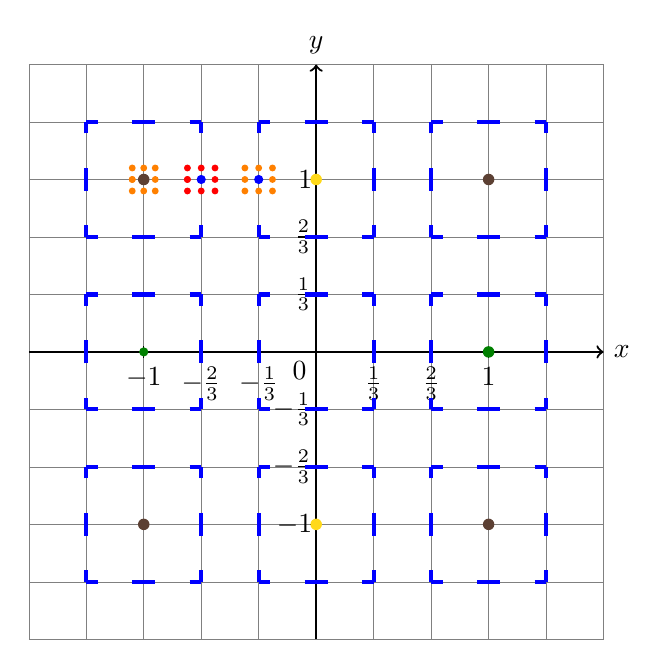
\begin{tikzpicture}[scale=0.73]
  % Draw grid
            \draw[step=1cm,gray,very thin] (-5,-5) grid (5,5);

            % Draw axes
            \draw[->,thick] (-5,0) -- (5,0) node[right] {$x$};
            \draw[->,thick] (0,-5) -- (0,5) node[above] {$y$};

            \draw (-3,0.1) -- (-3,-0.1) node[below] {$-1$};
            \draw (-2,0.1) -- (-2,-0.1) node[below] {$-\frac{2}{3}$};
            \draw (-1,0.1) -- (-1,-0.1) node[below] {$-\frac{1}{3}$};
            \draw (1,0.1) -- (1,-0.1) node[below] {$\frac{1}{3}$};
            \draw (2,0.1) -- (2,-0.1) node[below] {$\frac{2}{3}$};
            \draw (3,0.1) -- (3,-0.1) node[below] {$1$};
            \draw (-0.1, 3) -- (0.1, 3) node [left] {$1$};
            \draw (-0.1, 2) -- (0.1, 2) node [left] {$\frac{2}{3}$};
            \draw (-0.1, 1) -- (0.1, 1) node [left] {$\frac{1}{3}$};
            \draw (-0.1, -1) -- (0.1, -1) node [left] {$-\frac{1}{3}$};
            \draw (-0.1, -2) -- (0.1, -2) node [left] {$-\frac{2}{3}$};
            \draw (-0.1, -3) -- (0.1, -3) node [left] {$-1$};

            \node[below left] at (0,0) {0};

            % (-1,0)
            \fill[mydarkgreen, line width =1.5pt] (-3,0) circle (0.08cm);
            \draw [blue, line width=1.5pt] (-3.2, 1) -- (-2.8, 1); 

            \draw [blue, line width=1.5pt] (-2.2,1) -- (-2,1);
            \draw [blue, line width=1.5pt](-2, 1) -- (-2, 0.8);
            (-2,1) circle (0.08cm);

            \draw [blue, line width=1.5pt] (-2, 0.2) -- (-2,-0.2);
            (-2,0) circle (0.08cm);

            \draw [blue, line width=1.5pt] (-2, -0.8) -- (-2, -1);
            \draw [blue, line width=1.5pt] (-2.2, -1) -- (-2,-1);
            (-2,-1) circle (0.08cm);

            \draw [blue, line width=1.5pt] (-3.2, -1) -- (-2.8, -1);
            (-3,-1) circle (0.08cm);

            \draw [blue, line width=1.5pt] (-4,-1) -- (-3.8,-1);
            \draw [blue, line width=1.5pt] (-4, -1) -- (-4, -0.8);
            (-4,-1) circle (0.08cm);

            \draw [blue, line width=1.5pt] (-4, -0.2) -- (-4, 0.2);
            (-4,0) circle (0.08cm);

            \draw [blue, line width=1.5pt] (-4, 0.8) -- (-4, 1);
            \draw [blue, line width=1.5pt] (-4, 1) -- (-3.8, 1);
            (-4,1) circle (0.08cm);

            %(0,0)
            \draw [blue, line width=1.5pt](-0.2, 1) -- (0.2,1);
            (0,1) circle (0.08cm);

            \draw [blue, line width=1.5pt] (0.8,1) -- (1,1);
            \draw [blue, line width=1.5pt] (1, 1) -- (1, 0.8);
            (1,1) circle (0.08cm);

            \draw [blue, line width=1.5pt] (1, 0.2) -- (1,-0.2);
            (1,0) circle (0.08cm);


            \draw [blue, line width=1.5pt] (1, -0.8) -- (1, -1);
            \draw [blue, line width=1.5pt] (0.8, -1) -- (1, -1);
            (1,-1) circle (0.08cm);

            \draw [blue, line width=1.5pt] (-0.2, -1) -- (0.2, -1);
            (0,-1) circle (0.08cm);

            \draw [blue, line width=1.5pt] (-1, -1) -- (-0.8, -1);
            \draw [blue, line width=1.5pt] (-1, -1) -- (-1, -0.8);
            (-1,-1) circle (0.08cm);

            \draw [blue, line width=1.5pt] (-1, -0.2) -- (-1, 0.2);
            (-1,0) circle (0.08cm);

            \draw [blue, line width=1.5pt] (-1, 0.8) -- (-1, 1);
            \draw [blue, line width=1.5pt] (-1, 1) -- (-0.8, 1);
            (-1,1) circle (0.08cm);

            %(1,0)
            \fill [mydarkgreen, line width=1.5pt] (3,0) circle (0.1cm);

            \draw [blue, line width=1.5pt] (2.8,1) -- (3.2,1);
            (3,1) circle (0.08cm);

            \draw [blue, line width=1.5pt] (3.8,1) -- (4,1);
            \draw [blue, line width=1.5pt] (4, 1) -- (4, 0.8);
            (4,1) circle (0.08cm);

            \draw [blue, line width=1.5pt] (4, 0.2) -- (4,-0.2);

            \draw [blue, line width=1.5pt] (4, -0.8) -- (4, -1);
            \draw [blue, line width=1.5pt] (3.8, -1) -- (4, -1);

            \draw [blue, line width=1.5pt] (2.8, -1) -- (3.2, -1);

            \draw [blue, line width=1.5pt] (2, -1) -- (2.2, -1);
            \draw [blue, line width=1.5pt](2, -1) -- (2, -0.8);

            \draw [blue, line width=1.5pt](2, -0.2) -- (2, 0.2);

            \draw [blue, line width=1.5pt](2, 0.8) -- (2, 1);
            \draw [blue, line width=1.5pt](2, 1) -- (2.2, 1);

            %(-1,1)
            \fill[darkbrown] (-3,3) circle (0.1cm);

            %%%%%%%%%%%%%%%%%%%%%%%%%%%%%%%
            \fill [orange, line width=1.2pt] (-3.2, 3) circle (0.06cm);
            \fill [orange, line width=1.2pt] (-3.2, 3.2) circle (0.06cm);
            \fill [orange, line width=1.2pt] (-3, 3.2) circle (0.06cm);
            \fill [orange, line width=1.2pt] (-2.8, 3.2) circle (0.06cm);
            \fill [orange, line width=1.2pt] (-2.8, 3) circle (0.06cm);
            \fill [orange, line width=1.2pt] (-2.8, 2.8) circle (0.06cm);
            \fill [orange, line width=1.2pt] (-3, 2.8) circle (0.06cm);
            \fill [orange, line width=1.2pt] (-3.2, 2.8) circle (0.06cm);
            \fill [orange, line width=1.2pt] (-3.2, 3) circle (0.06cm);
            %%%%%%%%%%%%%%%%%%%%%%%%%%%%%%%

            \draw [blue, line width=1.5pt](-3.2, 4) -- (-2.8, 4); 

            \draw [blue, line width=1.5pt](-2.2, 4) -- (-2, 4);
            \draw [blue, line width=1.5pt](-2, 4) -- (-2, 3.8);

            \fill [blue, line width=1.5pt] (-2,3) circle (0.08cm);

            %%%%%%%%%%%%%%%%%%%%%%%%%%%%%%%
            \fill [red, line width=1.2pt] (-2.24, 3) circle (0.06cm);
            \fill [red, line width=1.2pt] (-2.24, 3.2) circle (0.06cm);
            \fill [red, line width=1.2pt] (-2, 3.2) circle (0.06cm);
            \fill [red, line width=1.2pt] (-1.76, 3.2) circle (0.06cm);
            \fill [red, line width=1.2pt] (-2.24, 3) circle (0.06cm);
            \fill [red, line width=1.2pt] (-1.76, 3) circle (0.06cm);
            \fill [red, line width=1.2pt] (-1.76, 2.8) circle (0.06cm);
            \fill [red, line width=1.2pt] (-2, 2.8) circle (0.06cm);
            \fill [red, line width=1.2pt] (-2.24, 2.8) circle (0.06cm);
            %%%%%%%%%%%%%%%%%%%%%%%%%%%%%%%

            \draw [blue, line width=1.5pt](-2, 2.2) -- (-2, 2);
            \draw [blue, line width=1.5pt](-2.2, 2) -- (-2, 2);

            \draw [blue, line width=1.5pt](-3.2, 2) -- (-2.8, 2);

            \draw [blue, line width=1.5pt](-4, 2) -- (-3.8, 2);
            \draw [blue, line width=1.5pt](-4, 2) -- (-4, 2.2);

            \draw [blue, line width=1.5pt](-4, 2.8) -- (-4, 3.2);

            \draw [blue, line width=1.5pt](-4, 3.8) -- (-4, 4);
            \draw [blue, line width=1.5pt](-4, 4) -- (-3.8, 4);

            %(-1,-1)
            \fill [darkbrown, line width=1.5pt] (-3,-3) circle (0.1cm);

            \draw [blue, line width=1.5pt](-3.2, -2) -- (-2.8, -2); 

            \draw [blue, line width=1.5pt](-2.2, -2) -- (-2, -2);
            \draw [blue, line width=1.5pt](-2, -2) -- (-2, -2.2);

            \draw [blue, line width=1.5pt](-2, -2.8) -- (-2, -3.2);

            \draw [blue, line width=1.5pt](-2, -3.8) -- (-2, -4);
            \draw [blue, line width=1.5pt](-2.2, -4) -- (-2, -4);

            \draw [blue, line width=1.5pt](-3.2, -4) -- (-2.8, -4);

            \draw [blue, line width=1.5pt](-4, -4) -- (-3.8, -4);
            \draw [blue, line width=1.5pt](-4, -4) -- (-4, -3.8);

            \draw [blue, line width=1.5pt](-4, -3.2) -- (-4, -2.8);

            \draw [blue, line width=1.5pt](-4, -2.2) -- (-4, -2);
            \draw [blue, line width=1.5pt](-4, -2) -- (-3.8, -2);

            %(1,1)
            \fill [darkbrown, line width=1.5pt] (3,3) circle (0.1cm);

            \draw [blue, line width=1.5pt](2.8,4) -- (3.2,4);

            \draw [blue, line width=1.5pt](3.8,4) -- (4,4);
            \draw [blue, line width=1.5pt](4, 4) -- (4, 3.8);

            \draw [blue, line width=1.5pt](4, 3.2) -- (4, 2.8);

            \draw [blue, line width=1.5pt](4, 2.2) -- (4, 2);
            \draw [blue, line width=1.5pt](3.8, 2) -- (4, 2);

            \draw [blue, line width=1.5pt](2.8, 2) -- (3.2, 2);

            \draw [blue, line width=1.5pt](2, 2) -- (2.2, 2);
            \draw [blue, line width=1.5pt](2, 2) -- (2, 2.2);

            \draw [blue, line width=1.5pt](2, 2.8) -- (2, 3.2);

            \draw [blue, line width=1.5pt](2, 3.8) -- (2, 4);
            \draw [blue, line width=1.5pt](2, 4) -- (2.2, 4);

            %(0,1)
            \fill [strongyellow, line width=1.5pt](0,3) circle (0.1cm);

            \draw [blue, line width=1.5pt](-0.2, 4) -- (0.2, 4);

            \draw [blue, line width=1.5pt](0.8, 4) -- (1, 4);
            \draw [blue, line width=1.5pt](1, 4) -- (1, 3.8);

            \draw [blue, line width=1.5pt](1, 3.2) -- (1, 2.8);

            \draw [blue, line width=1.5pt](1, 2.2) -- (1, 2);
            \draw [blue, line width=1.5pt](0.8, 2) -- (1, 2);

            \draw [blue, line width=1.5pt](-0.2, 2) -- (0.2, 2);

            \draw [blue, line width=1.5pt](-1, 2) -- (-0.8, 2);
            \draw [blue, line width=1.5pt](-1, 2) -- (-1, 2.2);

            \fill [blue, line width= 1.5pt] (-1,3) circle (0.08cm);

            %%%%%%%%%%%%%%%%%%%%%%%%%%%%%%%

            \fill [orange, line width=1.2pt] (-1.24, 3) circle (0.06cm);
            \fill [orange, line width=1.2pt] (-1.24, 3.2) circle (0.06cm);
            \fill [orange, line width=1.2pt] (-1, 3.2) circle (0.06cm);
            \fill [orange, line width=1.2pt] (-0.76, 3.2) circle (0.06cm);
            \fill [orange, line width=1.2pt] (-0.76, 3) circle (0.06cm);
            \fill [orange, line width=1.2pt] (-0.76, 2.8) circle (0.06cm);
            \fill [orange, line width=1.2pt] (-1, 2.8) circle (0.06cm);
            \fill [orange, line width=1.2pt] (-1.24, 2.8) circle (0.06cm);

            %%%%%%%%%%%%%%%%%%%%%%%%%%%%%%%

            \draw [blue, line width=1.5pt](-1, 3.8) -- (-1, 4);
            \draw [blue, line width=1.5pt](-1, 4) -- (-0.8, 4);

            %(0,-1)
            \fill [strongyellow, line width=1.5pt](0,-3) circle (0.1cm);
            \draw [blue, line width=1.5pt](-0.2, -2) -- (0.2, -2);

            \draw [blue, line width=1.5pt](0.8, -2) -- (1, -2);
            \draw [blue, line width=1.5pt](1, -2) -- (1, -2.2);

            \draw [blue, line width=1.5pt](1, -2.8) -- (1, -3.2);

            \draw [blue, line width=1.5pt](1, -3.8) -- (1, -4);
            \draw [blue, line width=1.5pt](0.8, -4) -- (1, -4);

            \draw [blue, line width=1.5pt](-0.2, -4) -- (0.2, -4);

            \draw [blue, line width=1.5pt](-1, -4) -- (-0.8, -4);
            \draw [blue, line width=1.5pt](-1, -4) -- (-1, -3.8);

            \draw [blue, line width=1.5pt](-1, -3.2) -- (-1, -2.8);

            \draw [blue, line width=1.5pt](-1, -2.2) -- (-1, -2);
            \draw [blue, line width=1.5pt](-1, -2) -- (-0.8, -2);

            %(1,-1)
            \fill[darkbrown, line width =1.5pt] (3,-3)circle (0.1cm);
            \draw [blue, line width=1.5pt](2.8, -2) -- (3.2, -2);

            \draw [blue, line width=1.5pt](3.8, -2) -- (4, -2);
            \draw [blue, line width=1.5pt](4, -2) -- (4, -2.2);

            \draw [blue, line width=1.5pt](4, -2.8) -- (4, -3.2);

            \draw [blue, line width=1.5pt](4, -3.8) -- (4, -4);
            \draw [blue, line width=1.5pt](3.8, -4) -- (4, -4);

            \draw [blue, line width=1.5pt](2.8, -4) -- (3.2, -4);

            \draw [blue, line width=1.5pt](2, -4) -- (2.2, -4);
            \draw [blue, line width=1.5pt](2, -4) -- (2, -3.8);

            \draw [blue, line width=1.5pt](2, -3.2) -- (2, -2.8);

            \draw [blue, line width=1.5pt](2, -2.2) -- (2, -2);
            \draw [blue, line width=1.5pt](2, -2) -- (2.2, -2);

    \end{tikzpicture}
    \caption{}
\end{center}
\end{figure}    
    It is still left to prove, that $h$ is open and continuous w.r.t. all three topologies. We will show it for $\tau_1$ and $\tau$. For $\tau_2$ it is similar as for $\tau_1$.\newline \newline
    First we observe the basis for $\tau_1$ is 
    $$\{(x - \frac{1}{3^{n_{(x,y)}}}, x +\frac{1}{3^{n_{(x,y)}}}) \times \{y\} \mid (x,y) \in X \times X\}$$
    and for $\tau$ is 
    $$\{(x - \frac{1}{3^{n_{(x,y)}}}, x +\frac{1}{3^{n_{(x,y)}}}) \times (y - \frac{1}{3^{n_{(x,y)}}}, y +\frac{1}{3^{n_{(x,y)}}}) \mid (x,y) \in X \times X\}$$
    We also observe that a basis for the topology on $T_{6,2,2}$ from $R_1$ is \{$B^1_t\}_{t \in T_{6,2,2}}$ where $B^1_t = \{s \in T_{6,2,2} \mid t R_1 s\}$ 
    and from $R$ is $\{B_t\}_{t \in T_{6,2,2}}$ where $B_t = \{s \in T_{6,2,2} \mid t R s\}$. The following arguments are carried over from Proposition 4.0.5. \newline
    Now, to see that $g$ is open w.r.t. $\tau_1$, we pick an open set $(x - \frac{1}{3^{n_{(x,y)}}}, x + \frac{1}{3^{n_{(x,y)}}}) \times \{y\} \in \tau_1$. 
    In similar way, we can show $g((x - \frac{1}{3^{n_{(x,y)}}}, x + \frac{1}{3^{n_{(x,y)}}}) \times \{y\}) = B^1_{g(x,y)}$. Thus $g$ is open.
    To show $g$ is continuous, it suffices to show that for each $t \in T_{6,2,2}$, the $g$-inverse image of $B^1_t$ belongs to $\tau_1$. Let $(x,y) \in g^{-1}(B^1_t)$. 
    Then $tR_1g(x,y)$. Hence, it holds for $(x,y)$ that $g((x - \frac{1}{3^{n_{(x,y)}}}, x + \frac{1}{3^{n_{(x,y)}}}) \times \{y\}) = B^1_{g(x,y)}$. By $t R_1g(x,y)$, we get
    $B^1_{g(x,y)} \subseteq B^1_t$. Thus, we found a neighborhood U of $(x,y)$ s.t. $U = ((x - \frac{1}{3^{n_{(x,y)}}}, x + \frac{1}{3^{n_{(x,y)}}}) \times \{y\}) \subseteq g^{-1}(B^1_t)$, implying $g$ is continuous.  \newline
    To see $g$ is open w.r.t. $\tau$, we pick pick an open set ($x- \frac{1}{3^{n_{(x,y)}}}, x+ \frac{1}{3^{n_{(x,y)}}}) \times (y- \frac{1}{3^{n_{(x,y)}}}, y+ \frac{1}{3^{n_{(x,y)}}})$. A similar argument as in Proposition 4.0.5, yields 
    us $g((x- \frac{1}{3^{n_{(x,y)}}}, x+ \frac{1}{3^{n_{(x,y)}}}) \times (y- \frac{1}{3^{n_{(x,y)}}}, y+ \frac{1}{3^{n_{(x,y)}}})) = B_{g(x,y)}$.

    

    \end{proof}

\end{theorem}



\clearpage
\section{Neighborhood}
\subsection{Neighborhood frames}

\begin{definition}
    Let $X$ be a non-empty set. A function  $\tau : X \rightarrow 2^{2^X}$ is called a neighbourhood function. A pair 
    F = (X,$\tau$) is called a neighbourhood frame (or n-frame). A model based on F is a tuple (X,$\tau$,v), where v assigns a subset of X to a variable
        
\end{definition}

\vspace{0.5cm}

\begin{definition}
    Let $M$ =($X$,$\tau$,v) be a neighourhood model and $x$ $\in$ $X$. The truth of a formula is defined inductively as follows :
    \begin{align*}
        M,x &\Vdash p \mbox{ iff } x \in V(p)\\
        M,x &\Vdash \neg \phi \mbox{ iff } M,x \nVdash \phi\\
        M,x &\Vdash \phi \lor \psi \mbox{ iff } M,x \vDash \phi \lor M,x \vDash \psi\\
        M,x &\Vdash \Box \phi \mbox{ iff } \exists V \in N(x) \forall y \in V : M,y \models \phi
    \end{align*}
    A formula is valid in a n-model $M$ if it is valid at all points of $M$ ($M \vDash \phi$). Formula is valid in a n-frame $F$ if it is valid in
    all models based on $F$ (notation $F \vDash \phi$). We write $F \vDash L$ if for any $\phi \in L, F \vDash \phi$. Logic of a class of n-frames $C$ as $Log(C) = \{\phi \mid F \vDash \phi \mbox{ for some } F \in C\}$
    $\mbox{We define nV(L) =  } \{ F \mid F \mbox{ is an n-frame and } F \models \phi \}$.
\end{definition}

\begin{definition}
    Let $X$ be a non-empty set and $\tau$ neighborhood function. We call $\tau$ is a filter if for each $x\in X$ the collection $\tau(x)$
    satisfies the following conditions : \newline \newline
    1. $\emptyset \notin \tau(x)$ \newline
    2. $\mbox{If }U \in \tau(x)$ and $U \subseteq V$ then $V \in \tau(x)$ (upward closed) \newline
    3. $\mbox{If }U, V \in \tau(x)$, then $U \cap V \in \tau(x)$
\end{definition}


\begin{definition}
    Let $F = (W,R)$ be a Kripke frame. We define an n-frame $N(F) = (W, \tau)$ as follows.
    For any $w\in W$ we have :
    $$\tau(w) = \{ U \mid R(w) \subseteq U \subseteq W \}$$
        
\end{definition}

\vspace{0.5cm}
\begin{lemma}

    Let $F = (W,R)$ be a Kripke frame. Then $$Log(F) = Log(N(F))$$ 
    The proof is by structural induction.
\end{lemma}

\vspace{0.5cm}

\begin{definition}
    Let $X$ = (X, $\tau_1$,...) and $Y$ = (Y, $\sigma_1$,...) be n-frames. Then the function $f$:
    $X \rightarrow Y$ is called bounded morphism if \newline \newline
    1. $f$ is surjective \newline
    2. $\forall x\in X \, \forall U \in \tau_i(x) : f(U) \in \sigma_i (f(x))$ \newline
    3. $\forall x\in X \, \forall V \in \sigma_i (f(x)) \, \exists U \in \tau_i(x) \, : f(U) \subseteq V$        
\end{definition}

\begin{corollary}
     Let $X$ = (X, $\tau_1$,...) and $Y$ = (Y, $\sigma_1$,...) be n-frames and $f : X \rightarrow Y$ a bounded morphism. Then 
     $$Log(X) \subseteq Log(Y)$$. \newline
     The proof is by structural induction.
\end{corollary}

\vspace{0.5cm}

\begin{definition}
    Let $X$ = (X, $\tau_1$) and $Y$ = (Y, $\tau_2$) be two n-frames. Then the product of these two frames
    is an n-2-frame and is defined as follows : \newline
    
    $$ X \times_n Y = (\mbox{X} \times \mbox{Y}, \tau_1', \tau_2')$$   
    $$ \tau_1'(x,y) = \{ U \subseteq \mbox{X} \times \mbox{Y} \mid \exists V \in \tau_1(x) : V \times  \{ y \} \subseteq U \}$$
    $$ \tau_2'(x,y) = \{ U \subseteq \mbox{X} \times \mbox{Y} \mid \exists V \in \tau_2(y) : \{ x \} \times V \subseteq U \}$$
    Additionally, we say the full product of n-frames $X \times^+_n Y$ is :
    $$ X \times^+_n Y = (X \times Y, \tau'_1, \tau'_2, \tau)\mbox{ where }$$
    $$ \tau(x,y) = \{ U \subseteq \mbox{X} \times \mbox{Y} \mid \exists W \in \tau_1(x) \, \exists V \in \tau_2(y) : W \times V \subseteq U \}$$        
\end{definition}

\begin{definition}
    For two unimodal logics $L_1$ and $L_2$ we define the n-product of them as follows :
    $$ L_1 \times_n L_2 = Log(\{ X \times Y \mid X \in nV(L_1) \mbox{ and } Y \in nV(L_2) \})$$        
\end{definition}

\begin{proposition}(\cite{?}).
    For two unimodal logics $L_1$ and $L_2$ it holds : 
    $$L_1 \otimes L_2 \subseteq L_1 \times_n L_2$$
\end{proposition}



\subsection{Main Construction}
In the following, we will construct a useful neighborhood frame called $N_\omega[F]$ based on a frame $F$.
We will use it later, to show $L_1 \times_n L_2 = L_1 \otimes L_2$ where $L_1,L_2 \in \{D,S4,D4,T\}$

\begin{definition}
    Let $F = (A^*, R) = F_{\xi \eta}[A]$ and $0 \notin A$. We define "pseudo-infinite" sequences 
    $$X = \{a_1a_2a_3... \mid a_i \in A \cup \{0\} \mbox{ and } \exists N \forall k \geq N : a_k = 0\}$$
    Furthermore, we define $f_F : X \rightarrow A^*$ to be the function, that deletes all zeros. \newline \newline
    Example : Say $12034002340^\omega \in X$ ($0^\omega$ denotes infinitely many zeros). Then $f_F(12034002340^\omega) = 1234234$

\end{definition}

\begin{definition}
    Let $F = (A^*, R) = F_{\xi \eta}[A]$ and $0 \notin A$. Assume the function $f_F$ and the set $X$ as defined before.
    For $\alpha \in X$ such that $\alpha = a_1a_2...$ we define 
    
    \begin{align*}
            st(a) &= min\{N \mid \forall k \geq N : a_k = 0\} \\
            a \mid_{k} &= a_1a_2...a_k \\
            U_k(\alpha) &= \{ \beta \mid f_F(\alpha)Rf_F(\beta) \mbox{ and } \alpha \mid_m = \beta \mid_m,  \mbox{ where } m = max((k, st(\alpha))\} 
    \end{align*} 
    Remark : Let $\alpha \in X \mbox{ with } st(\alpha) = n$. Then we have that $U_n(\alpha) = U_j(\alpha)$ for any $j \leq n$

\end{definition}

\begin{lemma}
    $U_k(\alpha) \subseteq U_m(\alpha)$, whenever $k \geq m$.
    
    \begin{proof}
        Let $\beta \in U_k(\alpha)$. Since $\alpha \mid_k = \beta \mid_k$ and $k \geq m$, we have $\alpha \mid_m = \beta \mid_m$. It follows, $\beta \in U_m(\alpha)$.
    \end{proof}
\end{lemma}

\begin{definition}
    Due to Lemma 5.2.3 the sets $U_n(\alpha)$ forms a filter base. So we can define :
    $$\tau(\alpha) \mbox{ is a filter with base } \{U_n(\alpha) \mid n \in \mathbb{N} \}$$
    $$N_\omega = (X, \tau) \mbox{ is the n-frame based on } F$$

\end{definition}

\begin{lemma}
    Let $F = (A^*, R) = F_{\xi \eta}[A]$. Based on that, let $N_\omega(F) = (X,\tau)$, $N(F) = (A^*, \sigma)$ and $f_F : N\omega(F) \rightarrow N(F)$.
    Then for any $m \in \mathbb{N}$ and $x\in X$ with $x = a_1a_2...$ \newline we have $$f_F(U_m(x)) = R(f_F(x))$$
    \vspace{0.01cm}
    \begin{proof}
            $\subseteq$ : Let $f_F(\alpha) \in f_F(U_m(x))$ with $\alpha \in U_m(x)$. By defintion of $U_m(x)$,
            we get $f_F(\alpha) \in R(f_F(x))$. \newline \newline
            For the other direction, we pick $\vec{a} \in R(f_F(x))$. We have to find $\beta \in U_m(x)$ s.t $f_F(\beta) = \vec{a}$. We assume R is irreflexive and non-transitive.
            The other cases are similar. \newline
            Because $\vec{a} \in R(f_F(x))$, there must exists $c \in A$ such that $ \vec{a} = f_F(x) * c $.
            We construct $\beta = x \mid_m \cdot \, c\, 0^\omega$. Hence, $f(\beta) = f_F(x \mid_m) * f_F(c)$ and because $ 0 \notin A$ we get $f_F(x \mid_m) * c = \vec{a}$.
            
            
    \end{proof}
\end{lemma}

\begin{lemma}
    Let $F =(A^*,R) = F_{\xi \eta}[A]$. Then $f_F : N_\omega(F) \rightarrow N(F)$ is a bounded morphism.

    \begin{proof}
        From now on this proof we will omit the subindex in $f_F$.
        Let $N_\omega(F) = (X, \tau)$ and $N(F) =(A^*, \sigma)$. \newline For surjectivity, we pick any $\vec{x} \in A^*$. But then, $\vec{x}\,0^\omega \in X$. Hence, $f(\vec{x}\, 0^\omega) = \vec{x}$. \newline 
        For the next condition, assume that $x \in X \mbox{ and } U \in \tau(x)$. We need to prove that $f(U) \in \sigma(f(x))$. That means $R(f(x)) \subseteq f(U)$. Because $U \in \tau(x)$, there is a $m$ such that
        $U_m(x) \subseteq U$. By Lemma 5.2.5 we have $f(U_m(x)) = R(f(x))$. It follows, 
        $$R(f(x)) = f(U_m(x)) \subseteq f(U)$$ 
        \newline
        Assume $x\in X$ and $V$ is a neighborhood of x, i.e $R(f(x)) \subseteq V$. We need to prove that there exists $U \in \tau(x)$, such that $f(U)\subseteq V$.
        As $U$ we $U_m(x)$ for any $m \in \mathbb{N}$. By Lemma 5.2.5 we get $f(U_m(x)) = R(f(x))$. Hence, 
        $$f(U_m(x)) = R(f(x)) \subseteq V$$

    \end{proof} 
\end{lemma}

\begin{corollary}
    For frame $F = F_{\xi \eta}[A]$ we have $Log(N_\omega(F)) \subseteq Log(F)$.
    \begin{proof}
        It follows from Lemma 5.1.5, Corollary 5.1.7 and Lemma 5.2.6 
        $$Log(N_\omega(F)) \subseteq Log(N(F)) = Log(F)$$
    \end{proof}

\end{corollary}

\begin{proposition}
    Let $F_{in} = F_{in}[\mathbb{N}], F_{rn} = F_{rn}[\mathbb{N}], F_{it} = F_{it}[\mathbb{N}] \mbox{ and } F_{rt} = F_{rt}[\mathbb{N}]$. Then
    $$Log(N_\omega(F_{in})) = D$$
    $$Log(N_\omega(F_{rn})) = T$$
    $$Log(N_\omega(F_{it})) = D4$$
    $$Log(N_\omega(F_{rt})) = S4$$

    \begin{proof}
        In all these cases, the inclusion from left to right follows from Proposition 2.1.9 and Corollary 5.2.7.
        Now the converse direction. Assume $X =(X,\tau)$. \newline
        It is easy to check that $X \vDash D$ iff for each $x \in X : \emptyset \notin \tau(x)$. For $N_\omega(F_{in})$ and $N_\omega(F_{it})$ this holds. \newline
        It is easy to check that $X \vDash T$ iff we have $x\in U \in \tau(x)$ for any $x$ and $U$. For $N_\omega(F_{rn})$ and $N_\omega(F_{rt})$ this holds. \newline
        Now we check $X \vDash 4$ iff for each $U \in \tau(x) : \{y \mid U \in \tau(y)\} \in \tau(x)$. \newline
        $\supseteq : $ Let $x \in X$ and assume $X,x \vDash \Box p$. That means there exists $U \in \tau(x)$ s.t $U\subseteq V(p)$.
        By assumption we have $S = \{y \mid U \in \tau(y)\} \in \tau(x)$. But then $X,x \vDash \Box\Box p$ because we can just pick the set S. \newline
        $\subseteq :$ By contradiction, assume there exists a $U$ s.t $\{y \mid U \in \tau(y)\} \notin \tau(x)$. Let $X,x \vDash \Box p$ where $V(p) = U$.
        If $X,x \vDash \Box\Box p$ then it must be the case that  \newline 
        $S =\{y \in X \mid X,y \vDash \Box p\} \in \tau(x)$. $X,y \vDash \Box p$ means $U \in \tau(y)$. That means $S = \{y \in X \mid U \in \tau(y)\}$. But by assumption $S \notin \tau(x)$. 
        Hence, $X,x \not\vDash \Box\Box p$. But thats a contradiction. This also holds for $N_\omega(F_{it})$ and $N_\omega(F_{rt})$ because we have for any $y \in U_m(x)$ and 
        $k \geq m : U_k(y) \subseteq U_m(x)$.
            
    \end{proof}
\end{proposition}

\begin{lemma}
    Let $T_{\omega,\omega,\omega[rn]}$ be as in Definition 3.2.1. Then 
    $$Log(T_{\omega,\omega,\omega[rn]}) = Log(N(T_{\omega,\omega,\omega[rn]}))$$ \newline
    The proof is by structural induction.

    
\end{lemma}

    Assume $F_1 = (A^*,R_1) = F_{\eta_1 \xi_1}[A]$ and $F_2 = (B^*,R_2) = F_{\eta_2 \xi_2}[B]$ 
    with $A \cap B = \emptyset$, $A = \{a_1,a_2,a_3,...\}$ and $B = \{b_1,b_2,b_3,...\}$. 
    Consider the product of n-frames $F'_1 = (X_1, \tau_1) = N_\omega(F_1)$ and $F'_2 = (X_2, \tau_2) = N_\omega(F_2)$ is 
    $$X = (X_1 \times X_2, \tau'_1, \tau'_2) = N_\omega(F_1) \times_n N_\omega(F_2)$$ \newline
    Furthermore, we have $F_1 \otimes F_2 = ((A \cup B)^*, R_1', R_2')$ as defined in Defintion 2.0.7.
    We consider the neighborhood version $$N(F_1 \otimes F_2) = ((A \cup B)^*, \sigma_1', \sigma_2')$$ \newline
    Now we define $g : X_1 \times X_2 \rightarrow (A \cup B)^*$ as follows. For $(\alpha, \beta) \in X_1 \times X_2$ with $\alpha = a_1a_2...$ and $\beta = b_1b_2...$
    we define $g(\alpha,\beta)$ to be the finite sequence which we get after eliminating all zeros from the infinite sequence
    $a_1b_1a_2b_2...$ \newline \newline
    Example : Let $\alpha = 012340^\omega$  and $\beta = 0ab00e0^\omega$. Then $g(\alpha, \beta) = 1a2b34e$.

\begin{lemma}
    Let $X$ and $N(F_1 \otimes F_2)$ be as defined before and $(\alpha,\beta) \in X_1 \times X_2$. Then for any $m >$ max$\{st(\alpha), st(\beta)\}$ we have 
    $$R_1'(g(\alpha,\beta)) = g(U_m(\alpha) \times \{\beta\})$$.

    \begin{proof}
        We will show both direction by assuming $F_1 = F_{in}[A]$. For $F_{it}[A],F_{rt}[A]$ and $F_{rn}[A]$ is it similar. \newline
        $\subseteq$ : Let $\vec{w} \in R'_1(g(\alpha,\beta))$. By definition we get, there exists $\vec{c} \in A^*$ where $\vec{w} = g(\alpha,\beta) \cdot \vec{c}$ and $\Lambda R_1 \vec{c}$.
        Because $R_1$ is irreflexive and non-transitive, we get $\vec{c} \in A$. We construct $(\zeta,\beta)$ where $\zeta \in U_m(\alpha)$ and $g(\zeta,\beta) = \vec{w}$. For that, we can take $\zeta = \alpha \mid_m \cdot \vec{c}\, 0^\omega$. Obviously, $\zeta \in U_m(\alpha)$.
        Because $m \in max\{st(\alpha), st(\beta)\}$, we have $g(\alpha \mid_m, \beta \mid_m) = g(\alpha, \beta)$. Hence, $g(\zeta, \beta) = g(\alpha \mid_m, \beta \mid_m) \cdot g(\vec{c} \,0^\omega, 0^\omega) = g(\alpha \mid_m, \beta \mid_m) \cdot \vec{c} = \vec{w}$.
        \newline \newline
        $\supseteq$ : Assume $\zeta \in U_m(\alpha)$. We have to show $g(\zeta, \beta) \in R_1'(g(\alpha, \beta))$. Because $R_1$ is irreflexive and non-transitive, it suffices to find a $\vec{c} \in A$ s.t. $g(\alpha,\beta) \cdot \vec{c} = g(\zeta, \beta)$.
        By choosing $m$ is maximal and $\zeta \mid_m = \alpha \mid_m$, we have $g(\zeta_m, \beta_m) = g(\alpha,\beta)$. We also know $f_F(\alpha)R_1 f_F(\zeta)$, that means there exists a $\vec{d} \in A$ s.t. $f_F(\alpha) \cdot \vec{c} = f_F(\zeta)$. This $\vec{d}$ must appear at a point after $\zeta_m$.
        We can follow $g(\zeta, \beta) = g(\alpha, \beta) \cdot \vec{d}$. Hence, $g(\zeta, \beta) \in R_1'(g(\alpha,\beta))$.
        \newline \newline
        Remark : If $m \leq max\{st(\alpha), st(\beta)\}$, then we cannot gurantee the equality. Assume $R_1$ as before and $\alpha = 123000^\omega$ and $\beta = d0b0a0^\omega$.
        Lets pick $m = 3$ and $\zeta = 123100^\omega$. Then we have $g(\alpha, \beta) = 1d23ba$ and $g(\zeta, \beta) = 1d23b1a$. Obviously, we don't have $g(\zeta, \beta) \in R_1'(g(\alpha,\beta))$. \newline
        Furthermore, we can show $R'_2(g(\alpha,\beta)) = g(\alpha \times U_m(\beta))$ similar as above. 
        
    \end{proof}


\end{lemma}

\begin{lemma}
    Function $g : X \rightarrow N(F_1 \otimes F_2)$ is a bounded morphism.

    \begin{proof}
        Let $\vec{z} = z_1z_2...z_n \in (A \cup B)^*$. Define for $i \leq n$ :
        \[
            x_i = 
            \begin{cases}
            z_i, & \text{if } z_i \in A; \\
            0, & \text{if } z_i \notin A.
            \end{cases}
            \qquad
            y_i = 
            \begin{cases}
            z_i, & \text{if } z_i \in B; \\
            0, & \text{if } z_i \notin B.
            \end{cases}
        \] \newline
        Let $\alpha = x_1x_2...x_n \, 0^\omega$ and $\beta = y_1y_2...y_n \, 0^\omega$. Then $g(\alpha,\beta) = \vec{z}$. Hence, g is surjective. \newline \newline
        For the next conditions we check only for $\tau_1'$ and $\sigma_1$. The other case is similar.
        Assume $(\alpha,\beta) \in X_1 \times X_2$ and $U \in \tau_1'(\alpha, \beta)$. We have to show $g(U) \in \sigma_1(g(\alpha,\beta))$. That means $R_1'(g(\alpha,\beta)) \subseteq g(U)$.
        Pick a $m > max\{st(\alpha), st(\beta)\}$ s.t. $U_m(\alpha) \times \{\beta\} \subseteq U$. We can pick such m, because $U \in \tau_1'(\alpha,\beta)$. So there exists $U_k(\alpha) \in \tau(\alpha)$ s.t. $U_k(\alpha) \times \{\beta\} = U$.
        If $k > max\{st(\alpha), st(\beta)\}$ then we are done. Else, by Lemma 5.2.3, we have for any $n \geq k : U_n(\alpha) \subseteq U_k(\alpha)$. So we can lift the $k$ til we reach $m$. Then we use Lemma 5.2.11 to get the following :
        $$R_1'(g(\alpha,\beta)) = g(U_m(\alpha) \times \{\beta\}) \subseteq g(U)$$
        \newline
        For the last condition we assume $(\alpha, \beta) \in X_1 \times X_2$ and $V \in \sigma_1(g(\alpha,\beta))$ (or rather $R_1'(g(\alpha,\beta)) \subseteq V$).
        We need to prove there exists $U \in \tau_1'(\alpha,\beta)$, such that $g(U) \subseteq V$. As $U$ we take $U_m(\alpha) \times \{\beta\}$ for some $m > max\{st(\alpha), st(\beta)\}$. Hence, by Lemma 5.2.11 we get :
        $$g(U_m(\alpha) \times \{\beta\}) = R_1'(g(\alpha,\beta)) \subseteq V$$ 
    \end{proof}
    
\end{lemma} 

    Now we will show $g : N_\omega(T_{\omega[rn]}) \times^+_n N_\omega(T_{\omega[rn]}) \rightarrow N(T_{\omega,\omega,\omega[rn]})$ is a bounded morphism. \newline 
    Let $(T_{\omega[rn]})_1 = (\mathbb{N}_{1}, R_1)$ and $(T_{\omega[rn]})_2 = (\mathbb{N}_{2}, R_2)$ as defined in Defintion 3.2.1.
    Then we take the n-frames $N_\omega(T_{\omega[rn]})_1 = (X_1, \tau_1)$ and $N_\omega(T_{\omega[rn]})_2 = (X_2, \tau_2)$. For the proof, we will omit the subscripts after the frame. \newline
    Let's consider the full product of the n-frames :
    $$N_\omega(T_{\omega[rn]}) \times^+_n N_\omega(T_{\omega[rn]}) = (X_1 \times X_2, \tau'_1, \tau'_2, \tau)$$
    \newline We say $N(T_{\omega,\omega,\omega[rn]}) = ((\mathbb{N}_1 \cup \mathbb{N}_2\cup \mathbb{N})^*, \sigma_1, \sigma_2, \sigma)$ where the tree $T_{\omega,\omega,\omega[rn]} = ((\mathbb{N}_1 \cup \mathbb{N}_2 \cup \mathbb{N})^*R_1',R_2',R)$ is as defined in Def.3.2.1\newline \newline
    In order to define the bounded morphism, we have to fix a bijection first. Let $h : \mathbb{N}_1 \times \mathbb{N}_2 \rightarrow \mathbb{N}$ be a bijection. \newline
    Next, we define function $k :(\mathbb{N}_1 \cup \{0\}) \times (\mathbb{N}_2 \cup \{0\}) \rightarrow \mathbb{N}_1 \cup \mathbb{N}_2 \cup \mathbb{N} \cup \{0\}$ as follows :
    \[
        f(a, b) =
        \begin{cases}
        a, & \text{if } b = 0; \\
        b, & \text{if } a = 0; \\
        h(a, b), & \text{otherwise}.
        \end{cases}
    \]

    Let $(\alpha,\beta) \in X_1 \times X_2$ with $\alpha = a_1a_2...$ and $\beta = b_1b_2...$. We define 
    $$g'(\alpha,\beta) = f(a_1,b_1)f(a_2,b_2)...$$
    At last, we define $g(\alpha,\beta)$ as $g'(\alpha,\beta)$ but removing all zeros.

    \begin{lemma}
        Function $g : N_\omega(T_{\omega[rn]}) \times^+_n N_\omega(T_{\omega[rn]}) \rightarrow N(T_{\omega,\omega,\omega[rn]})$ is a bounded morphism.
        
        \begin{proof}
            Let $\vec{z} = z_1z_2...z_n \in (\mathbb{N}_{1} \cup \mathbb{N}_{2} \cup \mathbb{N})^*$. We define for $i \leq n $
        \[
            x_i = 
            \begin{cases}
            z_i, & \text{if } z_i \in \mathbb{N}_{1}; \\
            a_1, & \text{if } z_i = h(a_1,b_2); \\
            0,   & \text{other}
            \end{cases}
            \qquad
            y_i = 
            \begin{cases}
            z_i, & \text{if } z_i \in \mathbb{N}_{2}; \\
            b_2, & \text{if } z_i = h(a_1,b_2); \\
            0,   & \text{other } 
            \end{cases}
        \] 
        \newline
        Let $\alpha = x_1x_2...x_n \, 0^\omega$ and $\alpha = y_1y_2...y_n \, 0^\omega$. But then $g(\alpha,\beta) = \vec{z}$. Hence, g is surjective.
        For the next conditions we show it for $\tau$ and $\sigma$. For $\tau_1', \sigma_1$ and $\tau_2', \sigma_2$ we can argue similar as in Lemma 5.2.11 and 5.2.12.\newline
        First we need to show, $R(g(\alpha,\beta)) = g(U_m(\alpha) \times U_m(\beta))$ for $m > max\{st(\alpha), st(\beta)\}$.
        The proof is similar as in Lemma 5.2.1. \newline
        $\supseteq$ : Pick $\zeta \in U_m(\alpha), \upsilon \in U_m(\beta)$. Show $g(\zeta, \upsilon) \in R(g(\alpha,\beta))$. By definition, we need to find a $\vec{c} \in \mathbb{N}_1 \cup \mathbb{N}_2 \cup \mathbb{N} \cup \{\epsilon\}$ s.t. $g(\alpha,\beta) \cdot \vec{c} = g(\zeta, \upsilon)$.
        By choosing $m> max\{st(\alpha),st(\beta)\}$, $\alpha \mid_m = \zeta \mid_m$ and $\beta \mid_m = \upsilon \mid_m$, we get $g(\alpha,\beta) = g(\zeta_m, \upsilon_m)$. Furthermore, we have $f_F(\alpha)R_1f_F(\zeta)$ and $f_F(\beta)R_2f_F(\upsilon)$, that means $\exists \vec{d} \in \mathbb{N}_1 \cup \{\epsilon\}$ and $\exists \vec{e} \in \mathbb{N}_2 \cup \{\epsilon\}$ s.t.
        $f_F(\alpha) \cdot \vec{d} = f_F(\zeta)$ and $f_F(\beta) \cdot \vec{e} = f_F(\upsilon)$. So, $\vec{d}$ must appear at a point after $\zeta \mid_m$. The same holds for $\vec{e}$ in $\upsilon$. But then we have $g(\zeta, \upsilon) = g(\alpha,\beta) * g(\vec{d}, \vec{e})$. Now there are four cases :
        \[
            \begin{cases}
            g(\vec{d}, \vec{e}) \in \mathbb{N}_1, & \text{if } \vec{d} \in \mathbb{N}_1 \text{ \&\ } \vec{e} = \epsilon \\
            g(\vec{d}, \vec{e}) \in \mathbb{N}_2, & \text{if } \vec{d} = \epsilon \text{ \&\ } \vec{e} \in \mathbb{N}_2\\
            g(\vec{d}, \vec{e}) \in \{\epsilon\}, & \text{if } \vec{d} =\vec{e} = \epsilon \\
            g(\vec{d}, \vec{e}) \in \mathbb{N}, & \text{other }
            \end{cases}
        \]
            Hence, $g(\zeta, \upsilon) \in R(g(\alpha,\beta))$. \newline \newline
            $\subseteq$ :  Pick $\vec{w} \in R(g(\alpha,\beta))$. We will construct $\zeta \in U_m(\alpha)$ and $\upsilon \in U_m(\beta)$ s.t. $g(\zeta,\upsilon) = \vec{w}$.
            By definition there exists a $\vec{c} \in \mathbb{N}_1 \cup \mathbb{N}_2 \cup \mathbb{N} \cup \{\epsilon\}$ s.t. $g(\alpha,\beta) \cdot \vec{c} = \vec{w}$. Depending on the $\vec{c}$,
            we build $\zeta = \alpha \mid_m \cdot \vec{d} \, 0^\omega$ and $\upsilon = \beta \mid_m \cdot \vec{e} \, 0^\omega$ where 

        \[
            \begin{cases}
            \vec{d} = \vec{c}, \vec{e} = 0, & \text{if }  \vec{c }\in \mathbb{N}_{1}; \\
            \vec{d} = 0, \vec{e} = \vec{c}, & \text{if }  \vec{c }\in \mathbb{N}_{2}; \\
            \vec{d} = \vec{e} = 0& \text{if } \vec{c }\in \{\epsilon\} \\
            \vec{d} = \vec{\alpha}, \vec{e} = \vec{b} \text{    where }h(\vec{\alpha},\vec{\beta}) = \vec{c} & \text{if } \vec{c } \in \mathbb{N} \, (\vec{\alpha} \in \mathbb{N}_1, \vec{\beta} \in \mathbb{N}_2);
            \end{cases}
        \] 
        \newline
        We have $\zeta \in U_m(\alpha)$ and $\upsilon \in U_m(\beta)$. Furthermore, because of $g(\zeta \mid_m, \upsilon \mid_m) = g(\alpha,\beta)$ it holds that $g(\zeta, \upsilon) = g(\alpha,\beta) \cdot g(\vec{d}, \vec{e}) = g(\alpha,\beta) \cdot \vec{c} = \vec{w}$. \newline \newline 
        Now to check the conditions, we assume $x \in X_1$ and $y \in X_2$ and $U \in \tau(x,y)$. We need to prove $g(U) \in \sigma(g(x,y))$ In other words, show $R(g(x,y)) \subseteq g(U)$. We pick a $m> max\{st(x),st(y)\}$ s.t. $U_m(x) \times U_m(y) \subseteq U$. But then we get 
        $$R(g(x,y)) = g(U_m(x) \times U_m(y)) \subseteq g(U)$$
        \newline
        Assume  $x \in X_1$ and $x \in X_2$ and $R(g(x,y)) \subseteq V$. We need to find a $U \in \tau(x,y)$, s.t. $f(U) \subseteq V$.
        For $U$ we pick $U_m(x) \times U_m(y)$ for some $m > \{st(x), st(y)\}$. But then 
        $$g(U_m(x) \times U_m(y)) = R(g(x,y)) \subseteq V$$

        \end{proof}
    \end{lemma}

    \subsection{Completeness Results}
    \begin{corollary}
        Let $F_1 = (A^*,R_1) = F_{\xi_1, \eta_1}[A]$ and $F_2 = (B^*,R_2) = F_{\xi_2, \eta_2}[B]$. Then 
        $$Log(N_\omega(F_1) \times_n N_\omega(F_2))  \subseteq Log(F_1) \otimes Log(F_2)$$.
        It follows from Proposition 2.1.8, Lemma 5.1.5, Corollary 5.1.7 and Lemma 5.1.12.
    \end{corollary}

    \begin{corollary}
        Let $F_1, F_2 \in \{F_{in}, F_{rn}, F_{it}, F_{rt}\}$. Then 
        $$Log(N_\omega(F_1) \times_nN_\omega(F_2)) = Log(F_1) \otimes Log(F_2)$$

        \begin{proof}
            The left to right inclusion follows from Corollary 5.3.1 \newline \newline
            To prove right to left, we know due to Proposition 2.1.9 and Proposition 5.2.8 we have $Log(N_\omega(F_i)) = Log(F_i) \, (i \in \{1,2\})$.
            Due to Proposition 5.1.10 we get $Log(N_\omega(F_1)) \otimes Log(N_\omega(F_2)) \subseteq Log(N_\omega(F_1)) \times_n Log(N_\omega(F_2))$. 
            Because $N_\omega(F_1)\times_n N_\omega(F_2)$ is a frame in the n-product, we get
            $Log(N_\omega(F_1)) \times_n Log(N_\omega(F_2)) \subseteq Log(N_\omega(F_1)\times_n N_\omega(F_2))$.

        \end{proof}

    \end{corollary}

    \begin{corollary}
        Let $N_\omega(T_{\omega[rn]})_1 = F_1$ and $N_\omega(T_{\omega[rn]})_2 = F_2$ as defined before. Then 
        $$T \times^+_n T \subseteq Log(T_{\omega,\omega,\omega[rn]})$$
        It follows from Corollary 5.1.7, Proposition 5.2.8, Lemma 5.2.9, Lemma 5.2.12

        \begin{proof}
            First, it is the case that $Log(F_1) \times^+_n Log(F_2) \subseteq Log(F_1 \times^+_n F_2)$. We can argue as before.
            By Lemma 5.2.12 it holds $Log(F_1) \times^+_n Log(F_2) \subseteq Log(N(T_{\omega,\omega,\omega[rn]})) = Log(T_{\omega,\omega,\omega[rn]})$.
            But by Proposition 5.2.8 we have $Log(F_1) = Log(F_2) = T$. Hence, $Log(F_1) \times^+_n Log(F_2) = T \times^+_n T \subseteq Log(T_{\omega,\omega,\omega[rn]})$.
        \end{proof}

    \end{corollary}

    \clearpage

    \begin{theorem}
        Let $L_1, L_2 \in \{S4, D4, D, T\}$. Then 
        $$L_1 \times_n L_2 = L_1 \otimes L_2$$

        \begin{proof}
            Right to left is by Proposition 5.1.10. \newline
            For left to right, assume $L_1 = Log(F_1)$ and $L_2 = Log(F_2)$ for some $F_1, F_2 \in \{F_{in}, F_{rn}, F_{it}, F_{rt}\}$.
            It follows from Corollary 5.3.2 \newline
            $L_1 \times_n L_2 = Log(N_\omega(F_1)) \times^+_n Log(N_\omega(F_2)) \subseteq Log(N_\omega(F_1) \times^+_n N_\omega(F_2)) = Log(F_1 \otimes F_2) = Log(F_1) \otimes Log(F_2) = L_1 \otimes L_2$
        \end{proof}
    \end{theorem}

    \begin{theorem}
        Let $N_\omega(T_{\omega[rn]})_1 = F_1'$ and $N_\omega(T_{\omega[rn]})_2 = F_2'$ as defined before. Then 
        $$T \times^+_n T = T \otimes T \otimes T + \Box p \rightarrow \Box_1 p \land \Box_2 p$$

        \begin{proof}
            For left to right it is easy to check the axioms. We pick any frame $F_1$ and $F_2$ s.t.
            $F_1 \vDash T$ and $F_2 \vDash T$. We consider $F_1 \times^+_n F_2$ the full product and let $(x,y) \in F_1 \times^+_n F_2$. \newline
            Assume $F_1 \times^+_n F_2,(x,y) \vDash \Box_1 p$. By definition, there exists a $U \in \tau_1'(x,y)$ s.t $U \subseteq V(p)$.
            But we have $U \supseteq V \times \{y\}$ for some $V \in \tau(x)$. By assumption, $F_1 \vDash T$, so we can follow $x \in V$. Hence, $(x,y) \in V(p)$. For $\Box_2p \rightarrow p$ it's done similar. \newline Let's check $\Box p \rightarrow p$.
            Assume $F_1 \times^+_n F_2,(x,y) \vDash \Box p$. By definition there exists a $U \in \tau(x,y)$ s.t. $U \subseteq V(p)$. But $U \supseteq V \times W$ for some $V \in \tau_1(x)$ and $W \in \tau_2(y)$.
            Because of the assumption, we must have $x \in V$ and $y \in W$. Hence, $(x,y) \in V(p)$. It follows $F_1 \times^+_n F_2,(x,y) \vDash p$. \newline
            Now we check the extra axiom.  Assume $F_1 \times^+_n F_2,(x,y) \Vdash \Box p$. By definition, there exists a $U \subseteq V(p)$, where $U \supseteq V \times W$ with $V \in \tau_1(x)$ and $W \in \tau_2(y)$. By assumption, we get $y \in W$. That means $U \in \tau_1'(x,y)$ 
            because $U \supseteq V \times \{y\}$. The same argument we can apply to $\tau_2'(x,y)$. Hence, $F_1 \times^+_n F_2,(x,y) \vDash \Box_1 p \land \Box_2 p$. The rest is clear. \newline
            Now for the other direction, we apply Corollary 5.3.3 to get $T \times^+_n T \subseteq Log(T_{\omega,\omega,\omega[rn]})$. By Proposition 3.2.6 we have
            $Log(T_{\omega,\omega,\omega[rn]}) = TNL$. Hence, 
            $$T \times^+_n T \subseteq T \otimes T \otimes T + \Box p \rightarrow \Box_1 p \land \Box_2 p$$.
            

        \end{proof}
        
    \end{theorem}


    



\end{document}

